%*******************************************************************************
%****************************** Sixth Chapter *********************************
%*******************************************************************************

\chapter{Quantifying Human-Humanoid Imitation Activities} \label{chapter6}

%% **************************** Define Graphics Path **************************
%\ifpdf
%    \graphicspath{{chapter6/figs/raster/}{chapter6/figs/PDF/}{chapter6/figs/}}
%\else
%    \graphicspath{{chapter6/figs/vector/}{chapter6/figs/}}
%\fi
\graphicspath{{figs/chapter6/PDF/}}

\section{Introduction} 
Similarly as in Chapter \ref{chapter5}, in this Chapter, 
results for experiments of human-humanoid imitation activities, 
described in Section \ref{sec:experiment:hhi},  
are presented by including time series, minimum embedding parameters, 
the reconstructed state spaces (RSS) using 
uniform time-delay embedding technique (UTDE), 
recurrence plots (RP),
recurrent quantification analysis (RQA), and 
weaknesses and strengthens of RQA with 
three dimensional surface plots of RQA. 

Time series data for this experiment are described as follows:
\begin{itemize}

\item Twenty participants defined as $pN$ where $N$ is the number of 
	participant.

\item Three levels of smoothness for the normalised data 
(sg0zmuv, sg1zmuv and sg2zmuv), computed from two different filter 
lengths (29 and 159) with the same polynomial degree of 5 using the 
function \texttt{sgolay(p,n,m)} \citep{Rsignal},

\item Four window length size: 2-sec (100 samples), 5-sec (250 samples), 
	10-sec (500 samples) and 15-sec (750 samples), and 

\item Four velocities of arm movement activity: horizontal normal (HN), 
	horizontal faster (HF), vertical normal (VN) and 
	vertical faster (VF)
\end{itemize}
To make the visual comparison easier, time series for only 
three participants ($p01$, $p02$, $p03$) with a window length 
of 10 seconds (500 samples) are considered for the following results.
See Appendix \ref{appendix:f} for further results.

%\newpage
\section{Time series}
Figures \ref{fig:tsH} and \ref{fig:tsV}
show time series of horizontal arm movements using axis GyroZ 
and  vertical arm movements using axis GyroY. 
The remaining time series are presented in Appendix \ref{appendix:f:ts}.
%%---------------------------------(FIGURE)-------------------------------------
\begin{figure}
  \centering
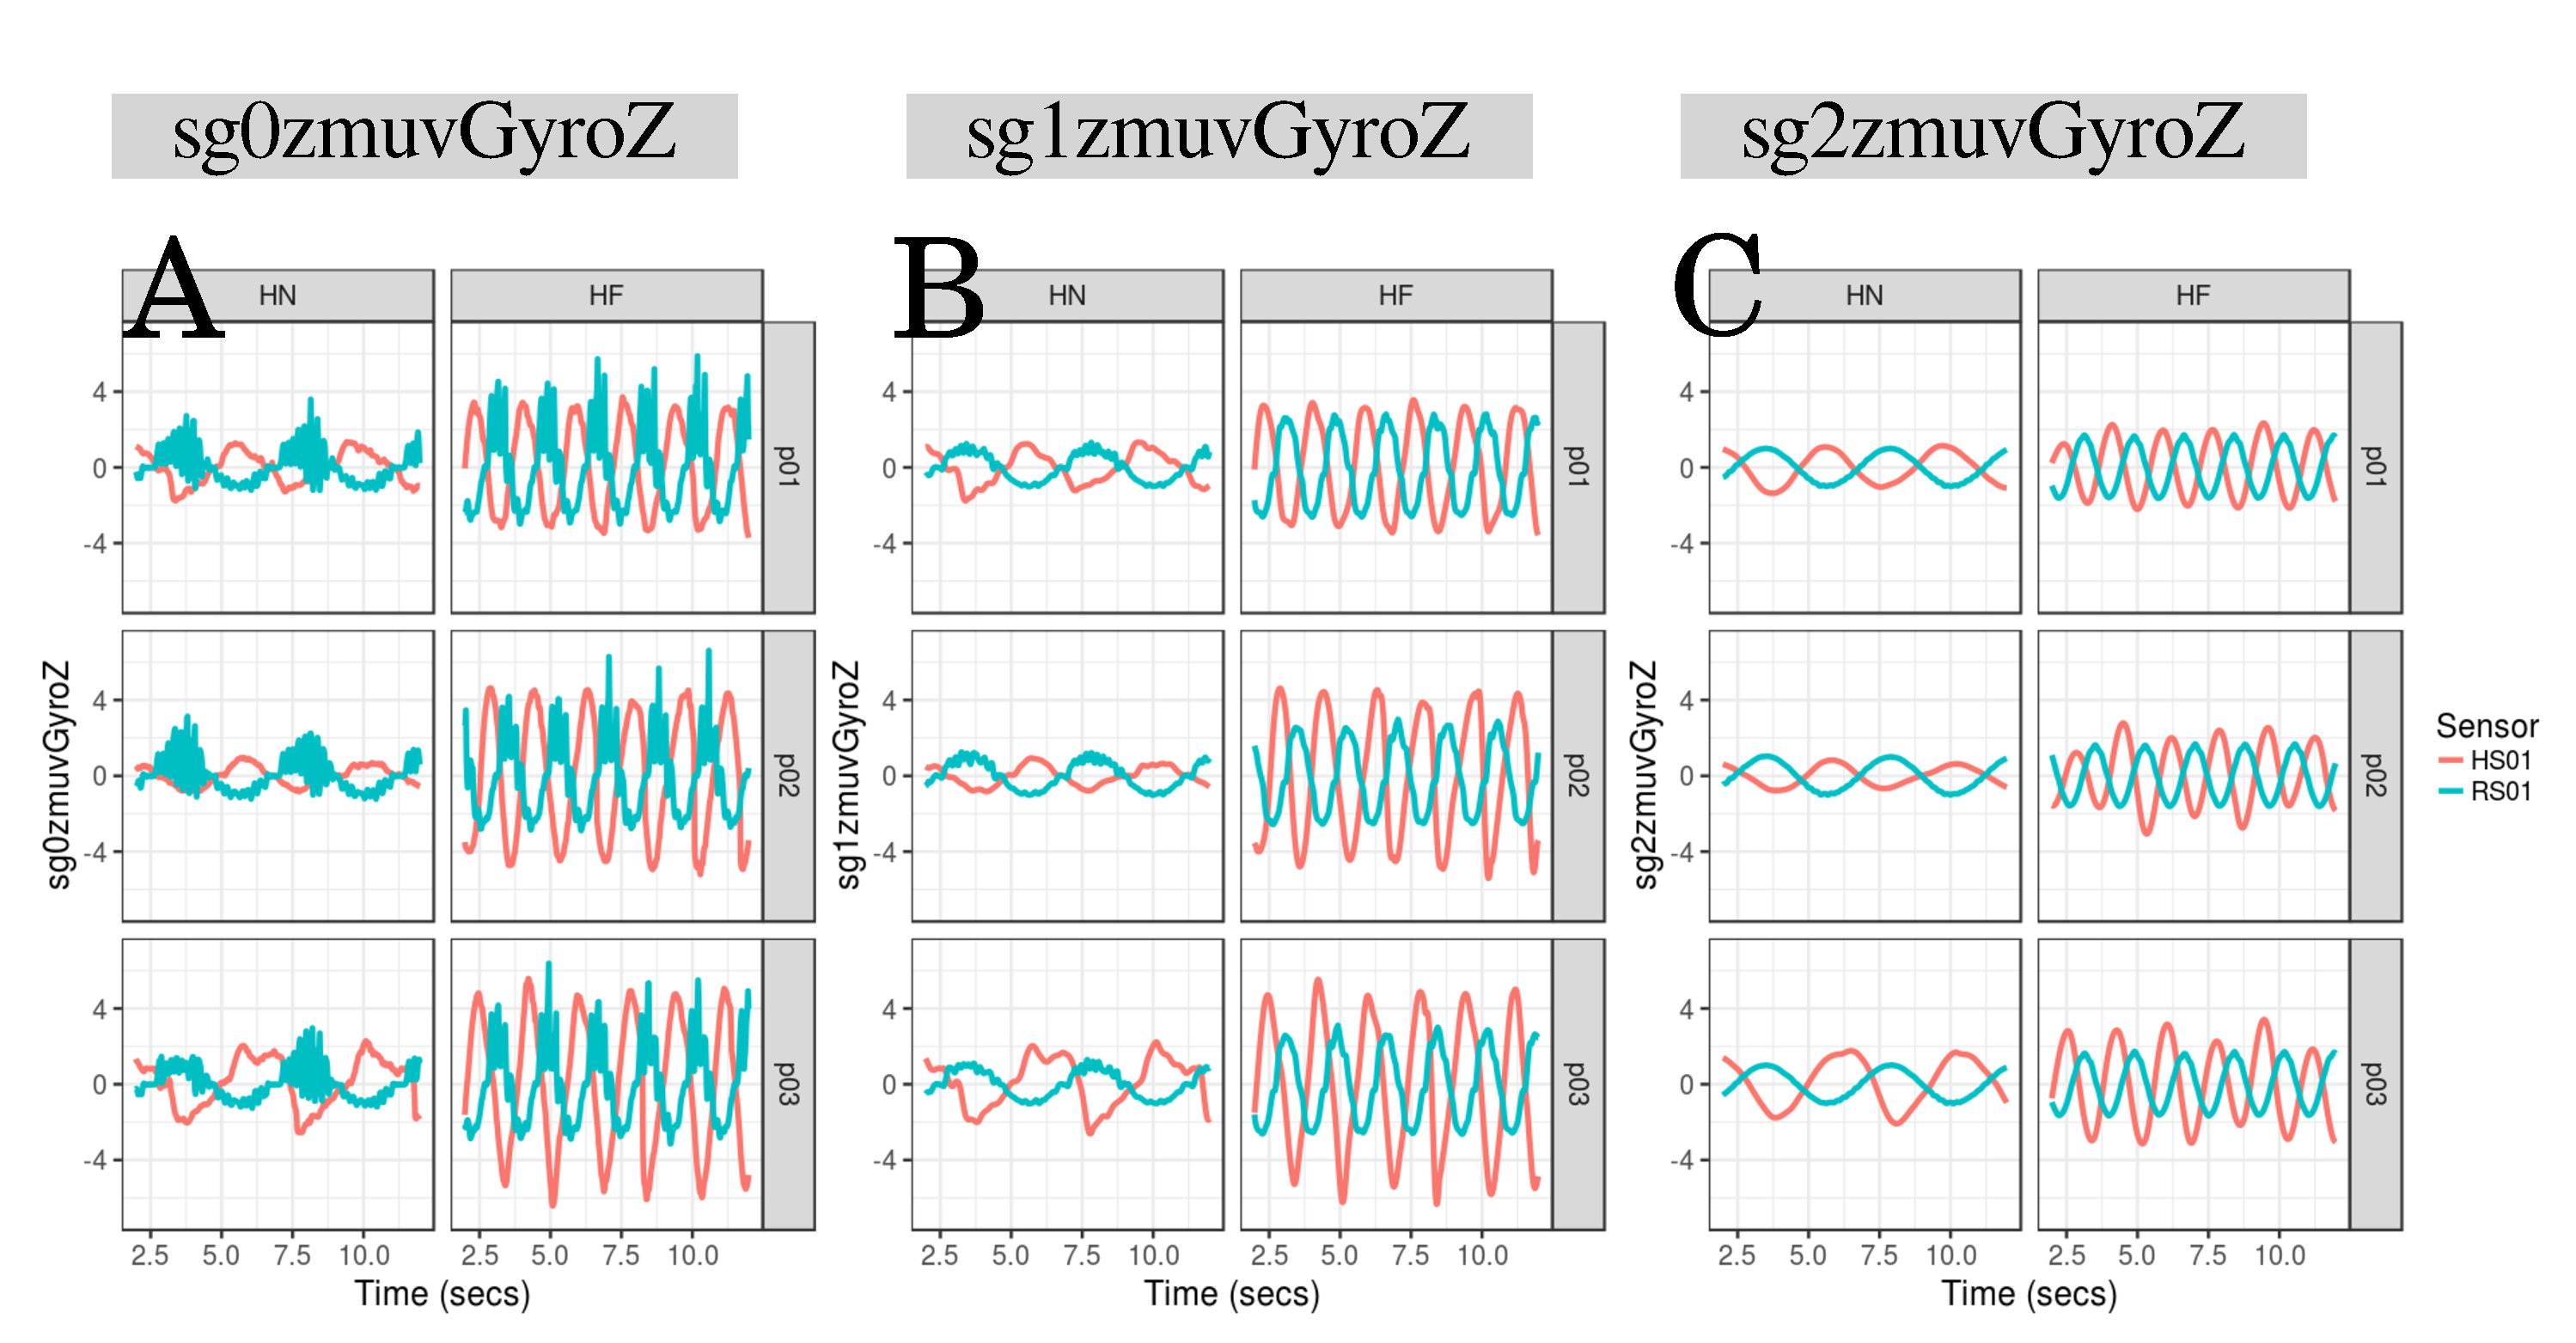
\includegraphics[width=1.0\textwidth]{fig_6_01}
    	\caption
	[Time series for horizontal arm movements]{
	{\bf Time series for horizontal arm movements.}
		(A) raw-normalised (sg0zmuvGyroZ), 
		(B) normalised-smoothed 1 (sg1zmuvGyroZ) and
		(C) normalised-smoothed 2 (sg2zmuvGyroZ).
		Time series are only for three participants 
		($p01$, $p02$, and $p03$) 
		for horizontal movements in normal and faster velocity (HN, HF) 
		with the normalised GyroZ axis (zmuvGyroZ) 
		and with one sensor attached to the participant (HS01) 
		and other sensor attached to the robot (RS01).	
	\R code to reproduce the figure is available at 
	\codelink{
	https://github.com/mxochicale-phd/thesis/tree/master/0_code_data/1_code/8_figs_ch6/01_fig6.1-6.2/code	
	}.
        }
    \label{fig:tsH}
\end{figure}
%%---------------------------------(FIGURE)------------------------------------
%%---------------------------------(FIGURE)-------------------------------------
\begin{figure}
  \centering
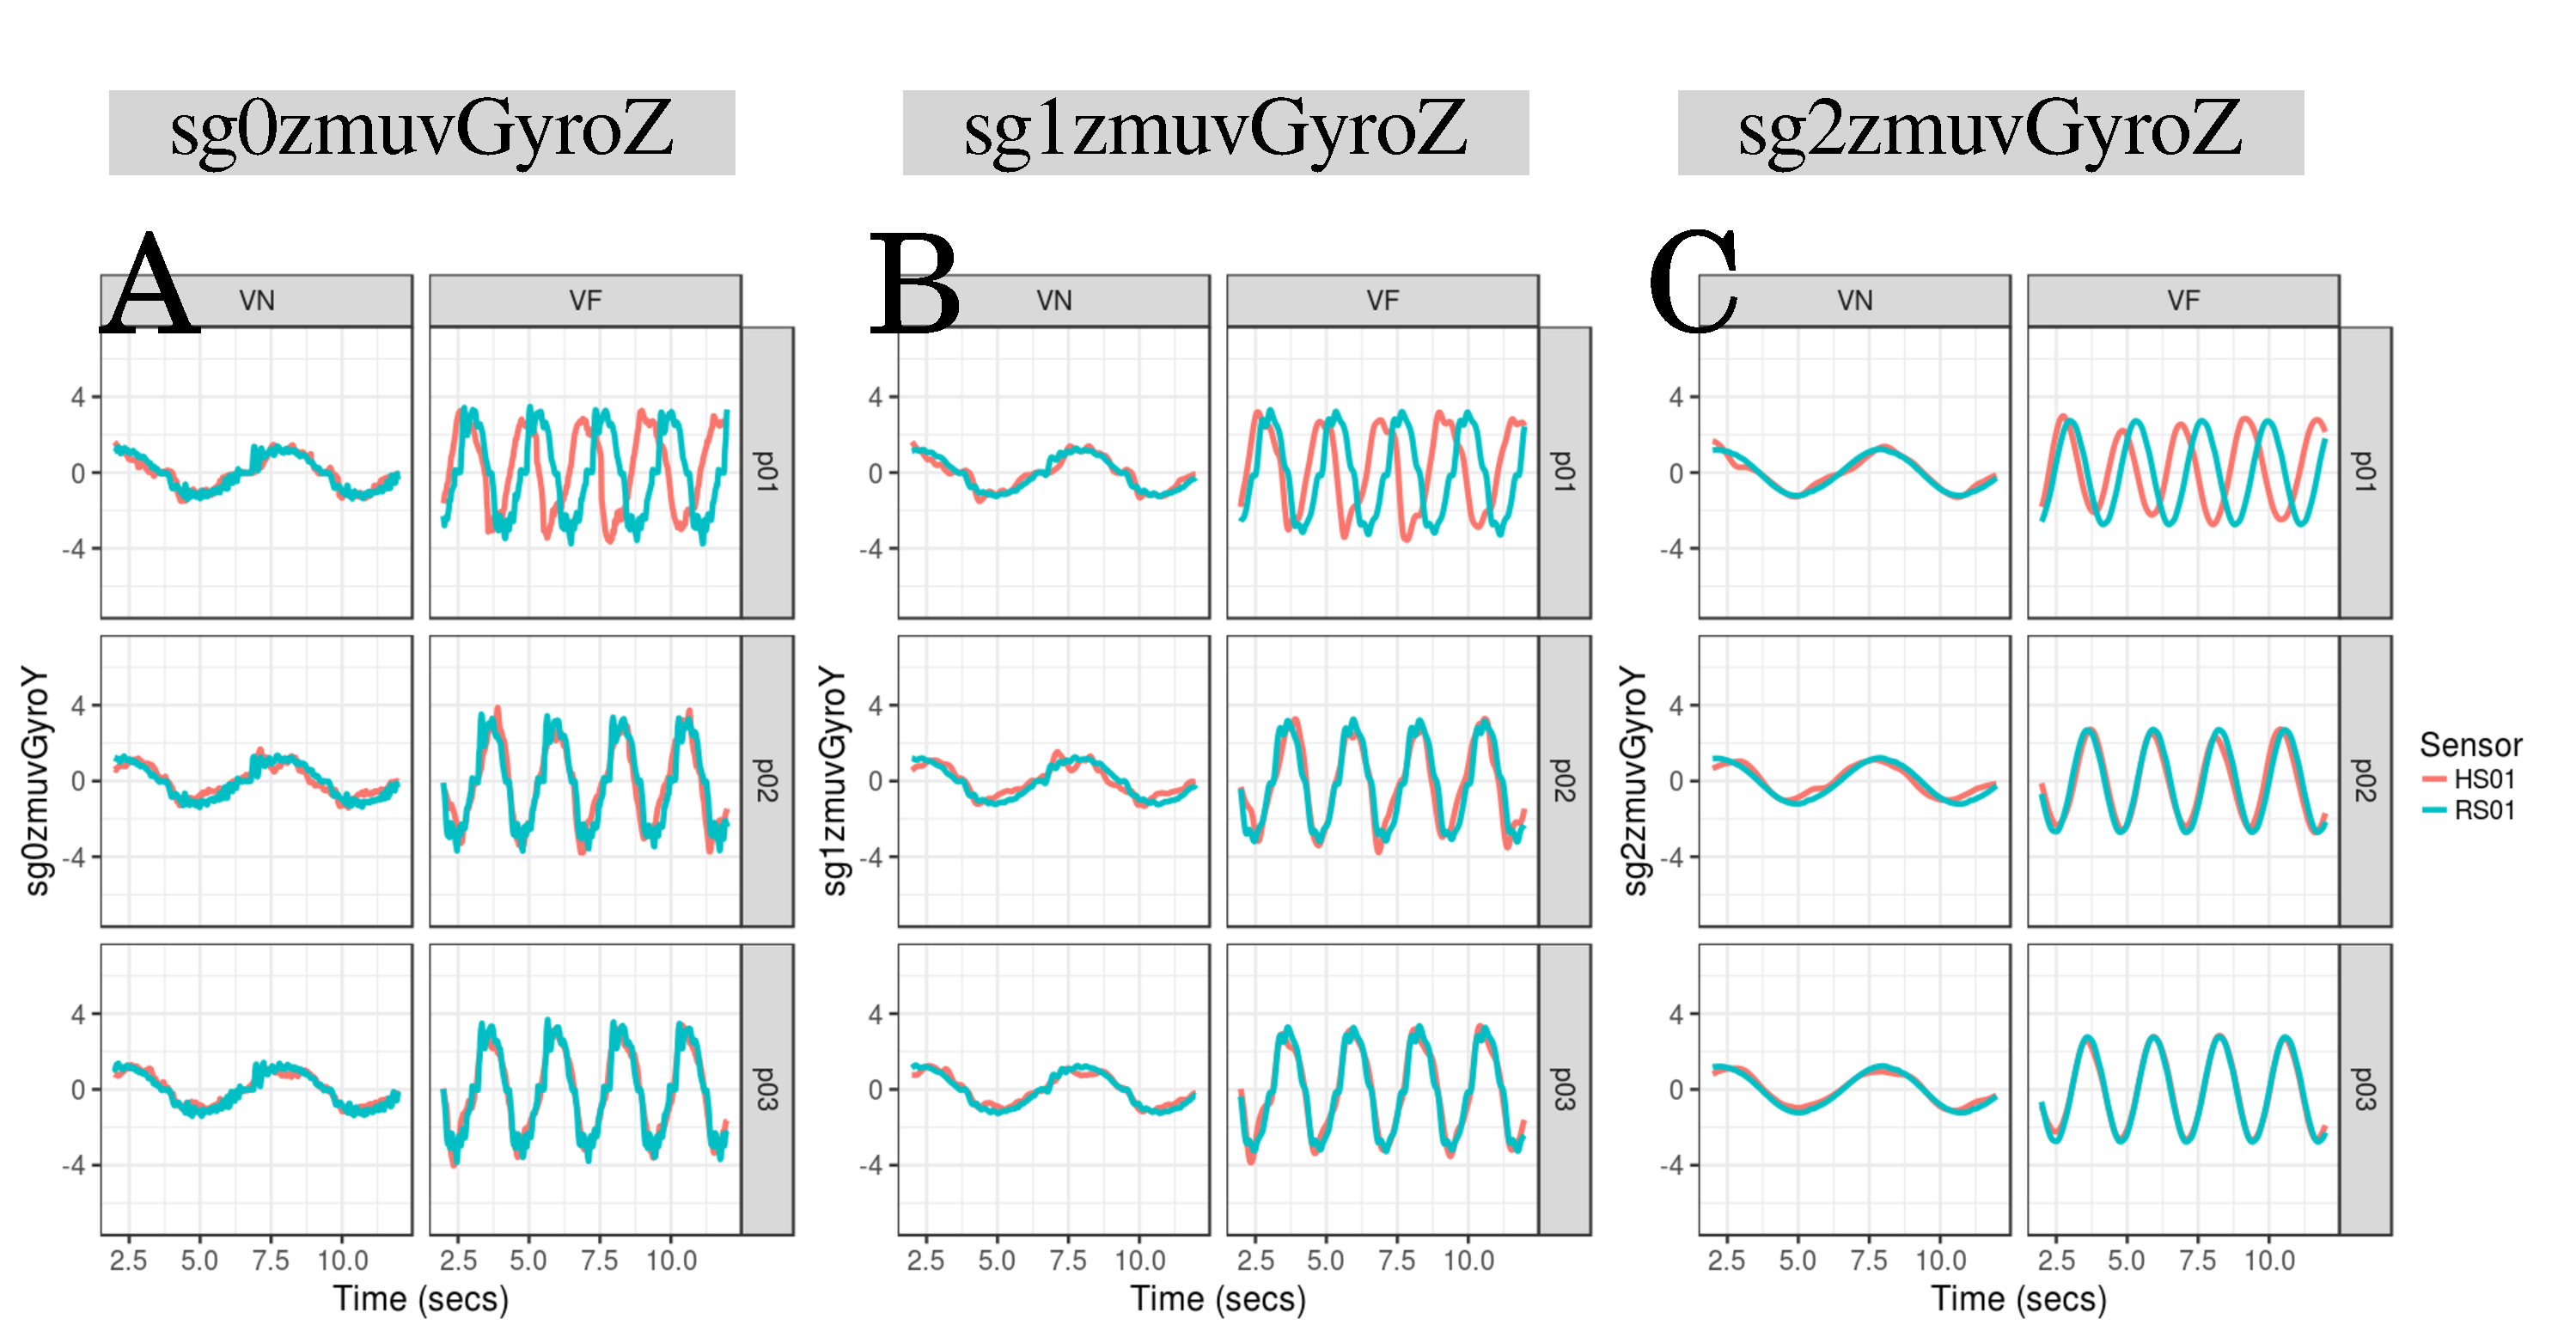
\includegraphics[width=1.0\textwidth]{fig_6_02}
	\caption
	[Time series for vertical arm movements]{
	{\bf Time series for vertical arm movements.}
		(A) raw-normalised (sg0zmuvGyroY), 
		(B) normalised-smoothed 1 (sg1zmuvGyroY) and
		(C) normalised-smoothed 2 (sg2zmuvGyroY).
		Time series are only for three participants 
		($p01$, $p02$, and $p03$) 
		for vertical movements in normal and faster velocity (VN, VF) 
		with the normalised GyroY axis (zmuvGyroY) 
		and with one sensor attached to the participant (HS01) 
		and other sensor attached to the robot (RS01).
	\R code to reproduce the figure is available at 
	\codelink{
	https://github.com/mxochicale-phd/thesis/tree/master/0_code_data/1_code/8_figs_ch6/01_fig6.1-6.2/code	
	}.
        }
    \label{fig:tsV}
\end{figure}
%%---------------------------------(FIGURE)------------------------------------

\newpage
\section{Minimum Embedding Parameters}
As mentioned in Section \ref{mep-hii} in Chapter \ref{chapter5}, 
minimum embedding parameters using FNN and AMI algorithms 
are computed for time series of this section.
Hence, Figs \ref{fig:CAOAMI-hhi}(A) show box plots of the minimum embedding 
dimensions of twenty participants performing horizontal and vertical arm
movements at normal and faster velocities (HN, HF, VN and VF) with 
attached sensors to participants (HS01) and to the robot (RS01).
Generally, Figs \ref{fig:CAOAMI-hhi}(A) show that minimum embedding values 
appear to be constant for sensor RS01 as their interquartile range 
in the box plots are near to 0.1 with the exception of two axis. 
Minimum embedding values for sensor HS01 appear to show more variations 
as their interquartile range of the box plots are near to 1 
with four exceptions.
Additionally, it can be seen in Figs \ref{fig:CAOAMI-hhi}(A) that there is a 
decrease of mean values (rhombus) in the box plots
as smoothness of time series increase. 
See Figs. \ref{fig:caoH} and \ref{fig:caoV} in Appendix \ref{appendix:f:ep} 
for detailed values of embedding dimensions for each participant.

Similarly, the first minimum values of AMI values 
for participants ($p01$ to $p20$), activities (HN, HF, VN, and VF) and 
sensors (HS01, RS01) are shown in the box plots of 
Figs \ref{fig:CAOAMI-hhi}(B).
It can be seen that values for HS01 tend to be more spread as the smoothness 
of the time series is increasing 
(see the increase of both mean (rhombus) and interquartile range).
However, AMI values for RS01 do not show such a similar increase in relation with
the increase of smoothness excepting for HF and VF
(see the increase of both mean (rhombus) and interquartile range) 
(Figs \ref{fig:CAOAMI-hhi}(B)).
Similarly to the minimum parameters in Chapter 5 (see \ref{mep-hii}),
there is a decrease of minimum embedding dimension as the smoothness 
is increasing, meaning that there is a decrease of the dynamics of 
the time series data. Also, the sample mean (gray rhombus) 
of first minimum AMI increase as the smoothness increase,
meaning that the maximal information to knowledge at $\tau_0$ 
also increase.
See Figs. \ref{fig:amiH} and \ref{fig:amiV} in Appendix \ref{appendix:f:ep} 
for more details about AMI values for each participant.
%%---------------------------------(FIGURE)-------------------------------------
\begin{figure}
\centering
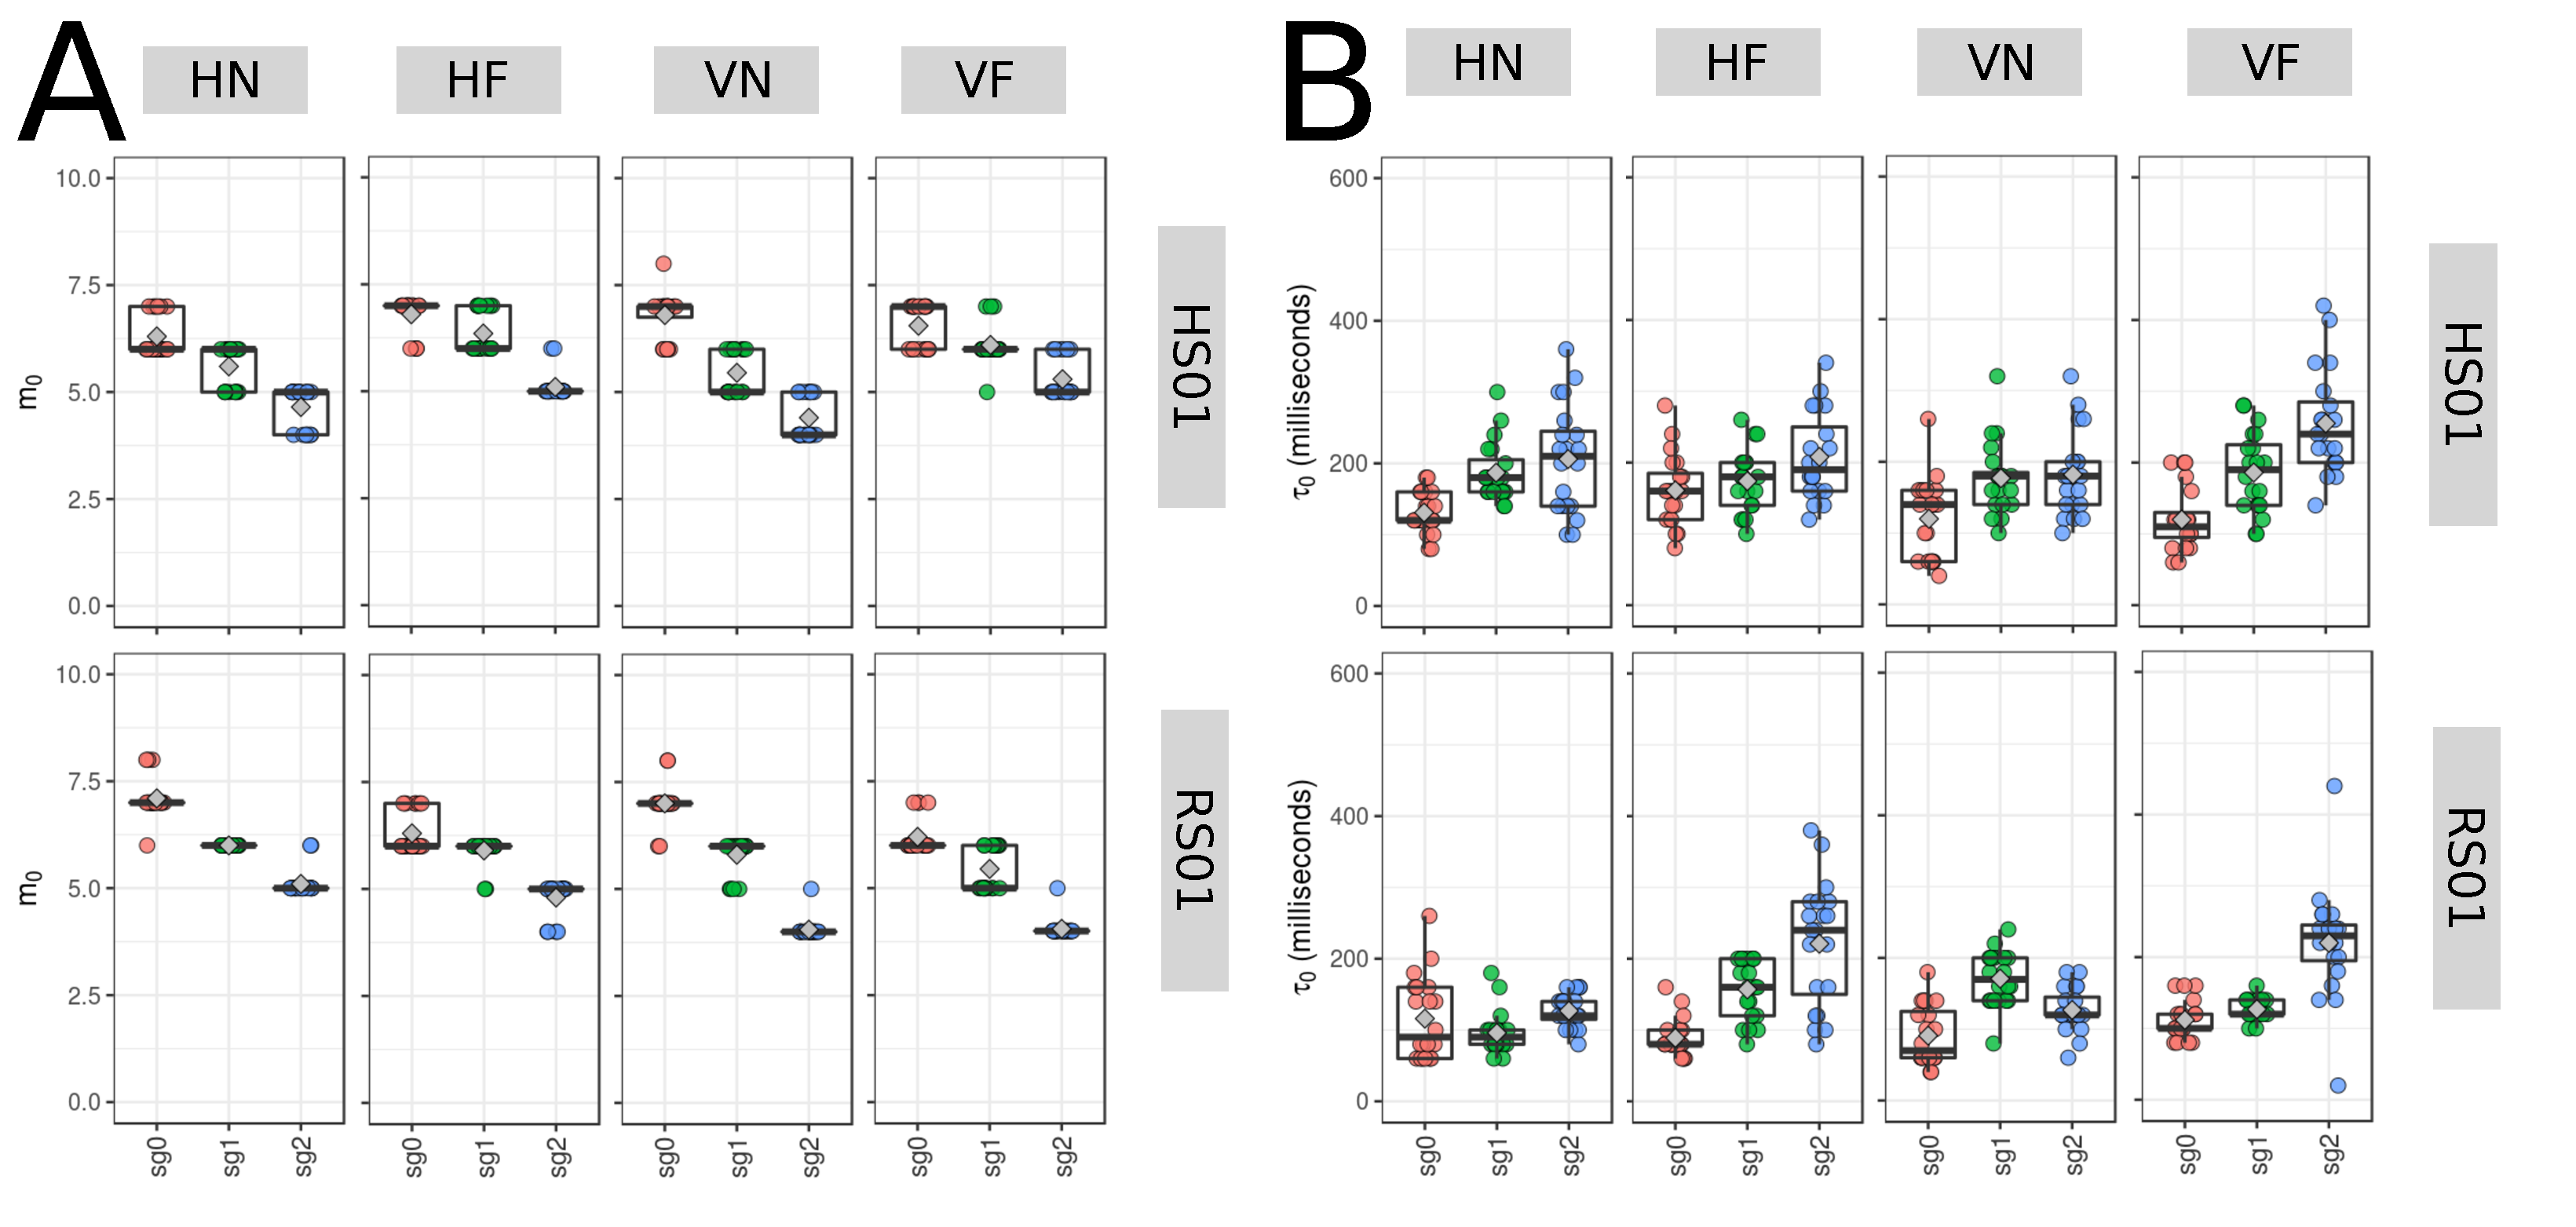
\includegraphics[width=1.0\textwidth]{fig_6_03}
	\caption
	[Box plots of minimum embedding parameters]{
	{\bf Box plots of minimum embedding parameters.} 
		Box plots of (A) minimum embedding dimensions 
		and (B) first minimum AMI values for 
		Horizontal Normal (HN), Horizontal Faster (HF),
		Vertical Normal (VN) and Vertical Faster (VF)
		with sensors attached to participants (HS01) and
		sensor attached to robot (RS01).
		Minimum embedding dimensions 
		($m_0$ and $\tau_0$)
		are for twenty participants 
		($p01$ to $p20$) with three smoothed signals 
		(sg0zmuvGyroZ (sg0) , sg1zmuvGyroZ (sg1) and sg2zmuvGyroZ (sg2))
		and window length of 10-sec (500 samples).
	\R code to reproduce the figure is available at 
	\codelink{
	https://github.com/mxochicale-phd/thesis/tree/master/0_code_data/1_code/8_figs_ch6/02_fig6.3/code
	}.
        }
    \label{fig:CAOAMI-hhi}
\end{figure}
%%---------------------------------(FIGURE)------------------------------------

\newpage
\subsection{Average minimum embedding parameters}
Following the Section \ref{sec:overall_minMT} to compute the overall average 
of minimum embedding parameters, the sample mean for the 
minimum values of $E_{1}(m)$ from Figs \ref{fig:CAOAMI-hhi}(A) 
is $\overline{m}_0=6$ and the sample 
mean for minimum values of AMIs from Figs~\ref{fig:CAOAMI-hhi}(B)
is $\overline{\tau}_0=8$, for which the overall average minimum embedding 
parameters is ($\overline{m_0}=6$, $\overline{\tau_0}=8$).
Hence, the average minimum embedding parameters 
($\overline{m_0}=6$, $\overline{\tau_0}=8$)
has been considered to compute 
Reconstructed State Spaces (RSSs), Recurrence Plots (RPs) and
Recurrence Quantification Analysis (RQA) metrics for human-humanoid activities.

\section{Reconstructed state spaces with UTDE}
Considering Section \ref{sec:rsswithUTDE} and time series for participant $p01$ 
(Figs \ref{fig:tsH}, \ref{fig:tsV}) the reconstructed state spaces
for horizontal arm movements (Figs~\ref{fig:rss_aHw10}) and
 vertical arm movements  (Figs~\ref{fig:rss_aVw10}) 
are computed with $\overline{m_0}=6$ and $\overline{\tau_0}=8$ 

The trajectories of the RSSs for horizontal normal and faster from 
HS01 and RS01 are slightly smoothed as the time-series 
smoothness increase (Figs~\ref{fig:rss_aHw10}). 
Although the frequency of the movement increase from normal to faster velocity
activities, the trajectories RSSs in Figs~\ref{fig:rss_aHw10}(B)
show highers oscillations specially for a maximum values of smoothness
(sg2zmuvGyroZ), while the trajectories in the RSS for HF in 
Figs~\ref{fig:rss_aHw10}(D) show a lower and smoothed oscillations 
as the smoothness increase.
In contrast, the time series for vertical movements are less noisy and 
well structured (Figs \ref{fig:tsV}) for which the trajectories in the RSSs 
seem to be less organised, specially for Fig \ref{fig:rss_aVw10}(A,C), 
while time series for vertical faster movements (VF) which have more 
periods (Figs \ref{fig:tsV}) present trajectories in the RSS with 
well defined patters (\ref{fig:rss_aVw10}(C,D)).
It is important to note that the smoothness of time series also create 
an effect on smoothness in the trajectories of the RSS, being the RS01 
more organised and more persistent while trajectories for HS01 are 
more changeable (Figs. \ref{fig:rss_aHw10}, \ref{fig:rss_aVw10}).

%%---------------------------------(FIGURE)-------------------------------------
\begin{figure}
\centering
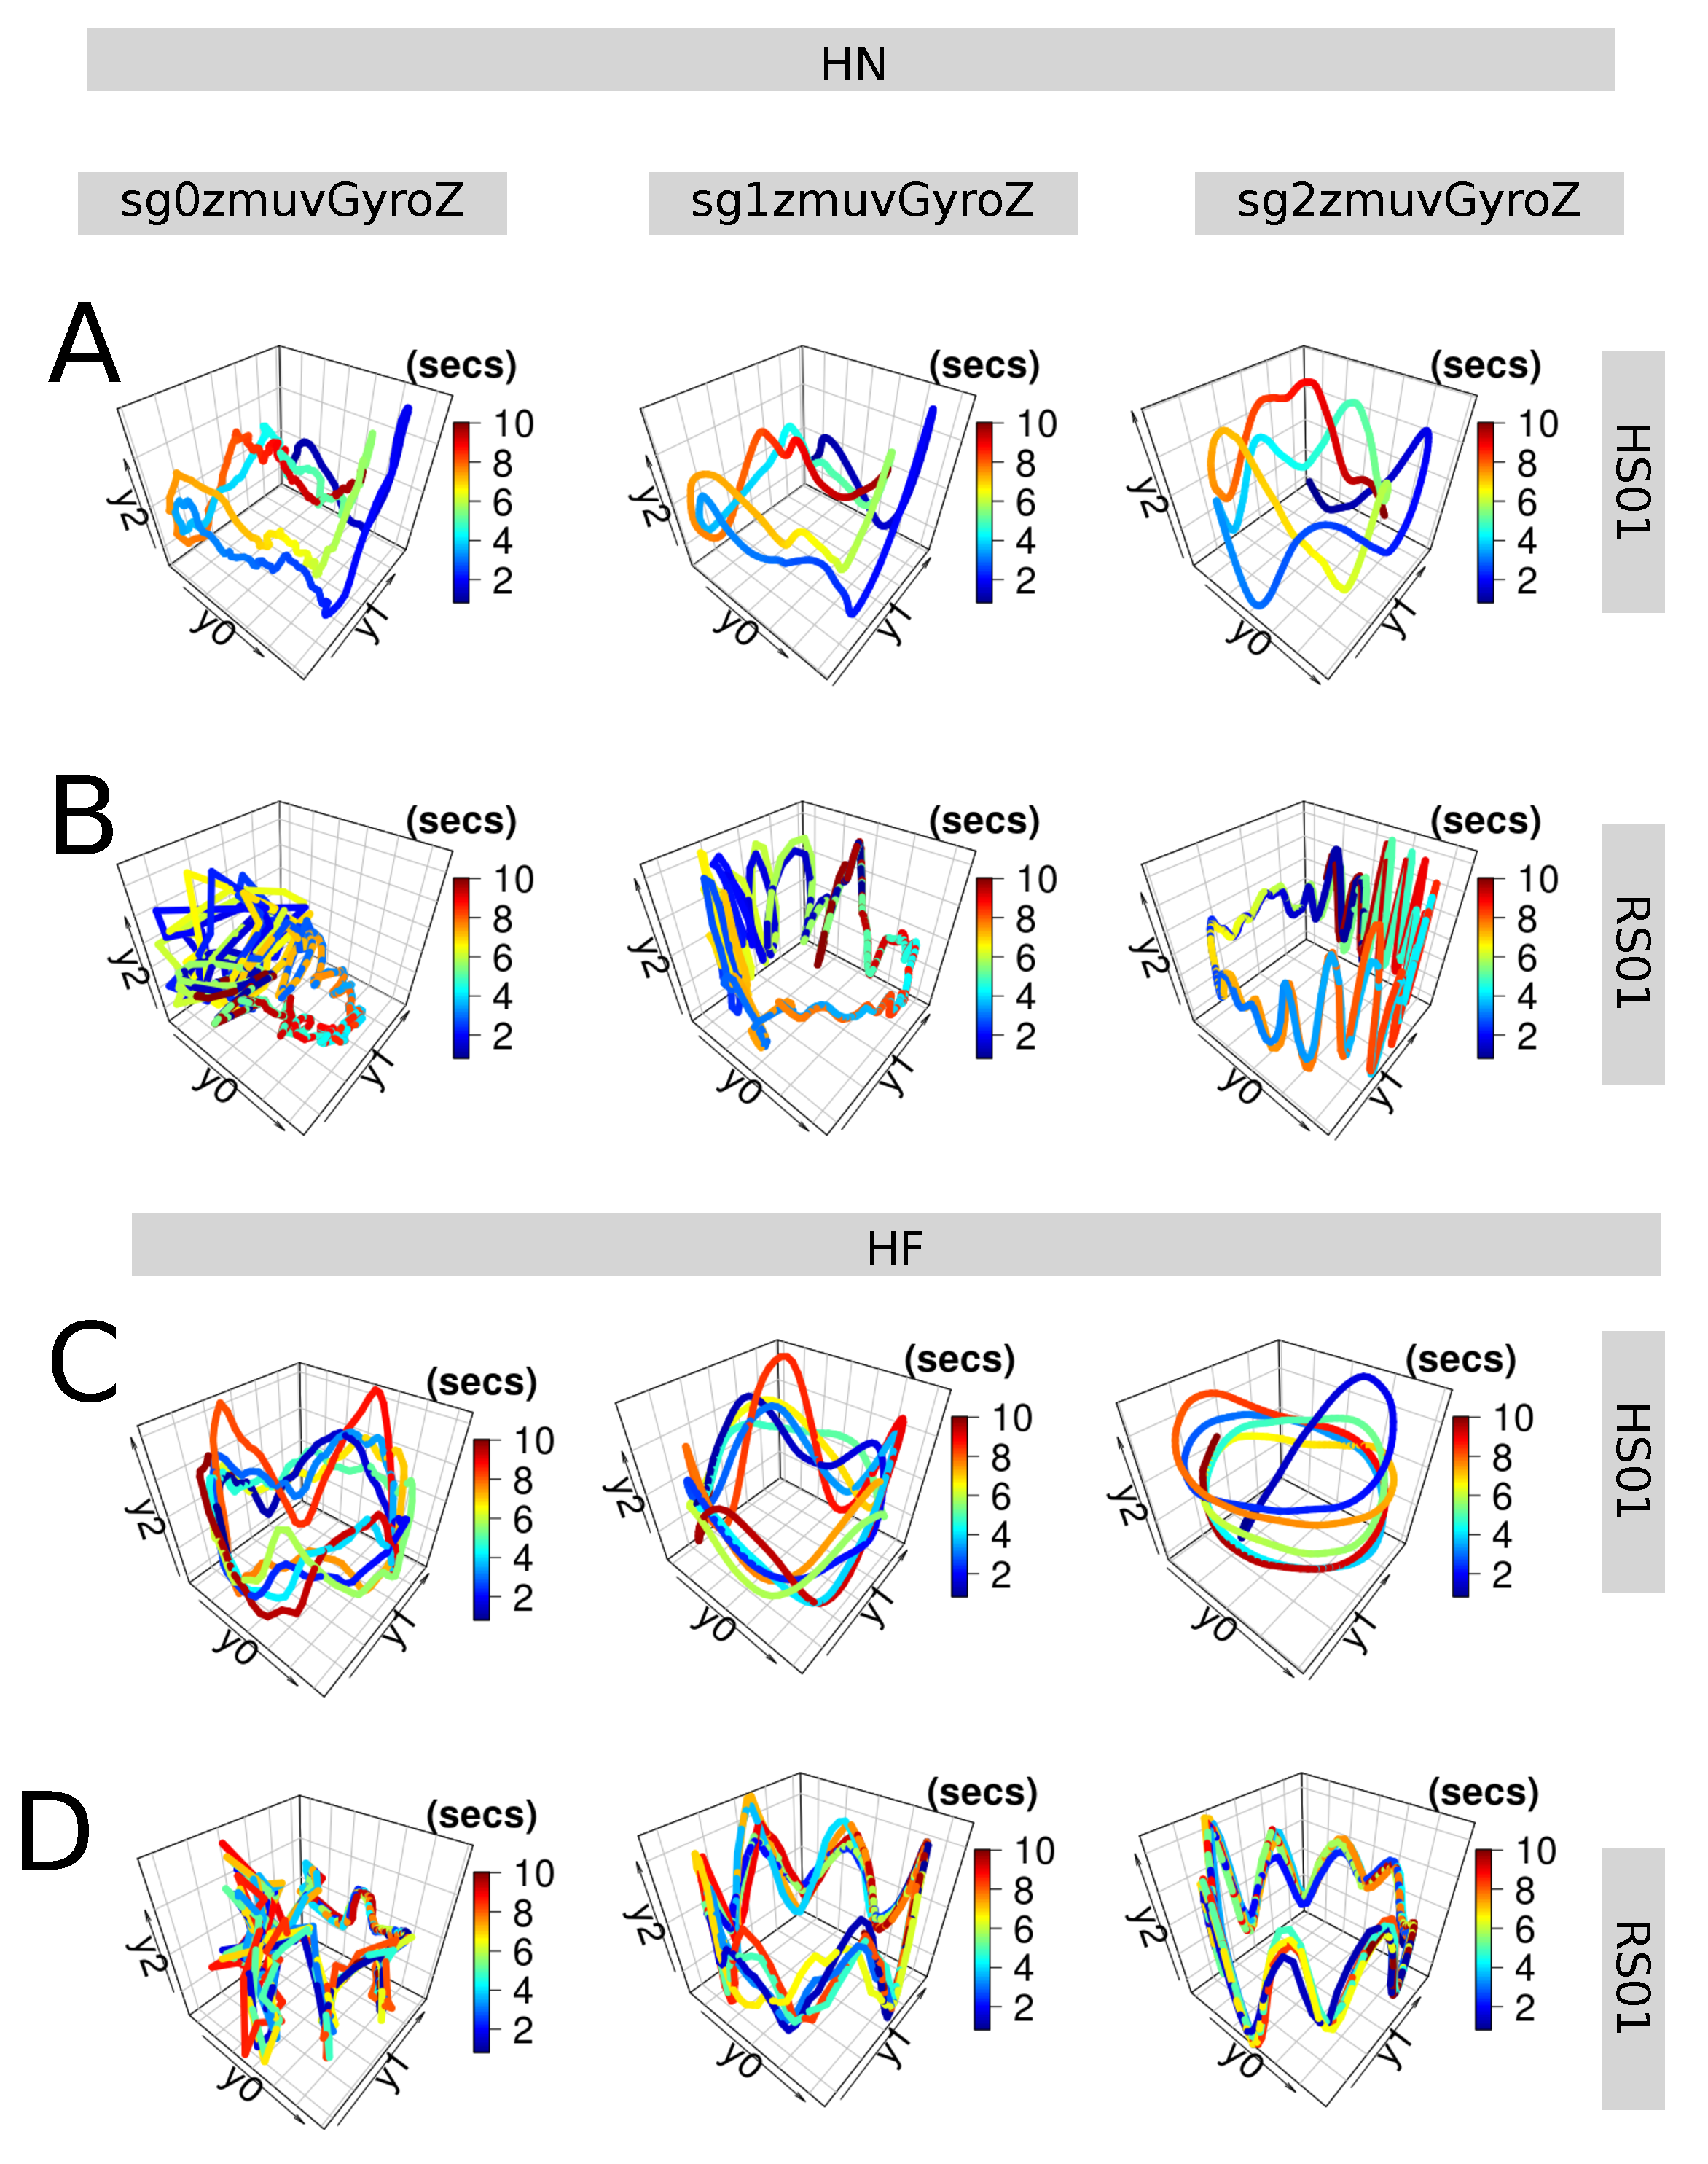
\includegraphics[height=0.85\textheight]{fig_6_04}
\caption
	[RSSs for horizontal arm movements]{
	{\bf RSSs for horizontal arm movements.}
	Reconstructed state spaces %for time series of Figure \ref{fig:tsH}.
	of participant p01 for horizontal movements in normal and faster 
	velocity (HN, HF) with raw-normalised (sg0zmuvGyroZ), 
	normalised-smoothed 1 (sg1zmuvGyroZ) and 
	normalised-smoothed 2 (sg2zmuvGyroZ) time series of the 
	sensors attached to the participant (HS01) and other sensor 
	attached to the robot (RS01).	
	Reconstructed state spaces were computed with 
	embedding parameters $\overline{m_0}=6$, $\overline{\tau_0}=8$.
	\R code to reproduce the figure is available at 
	\codelink{
	https://github.com/mxochicale-phd/thesis/tree/master/0_code_data/1_code/8_figs_ch6/03_fig6.4-6.5
	}.
        }
    \label{fig:rss_aHw10}
\end{figure}
%%---------------------------------(FIGURE)------------------------------------

%%---------------------------------(FIGURE)-------------------------------------
\begin{figure}
\centering
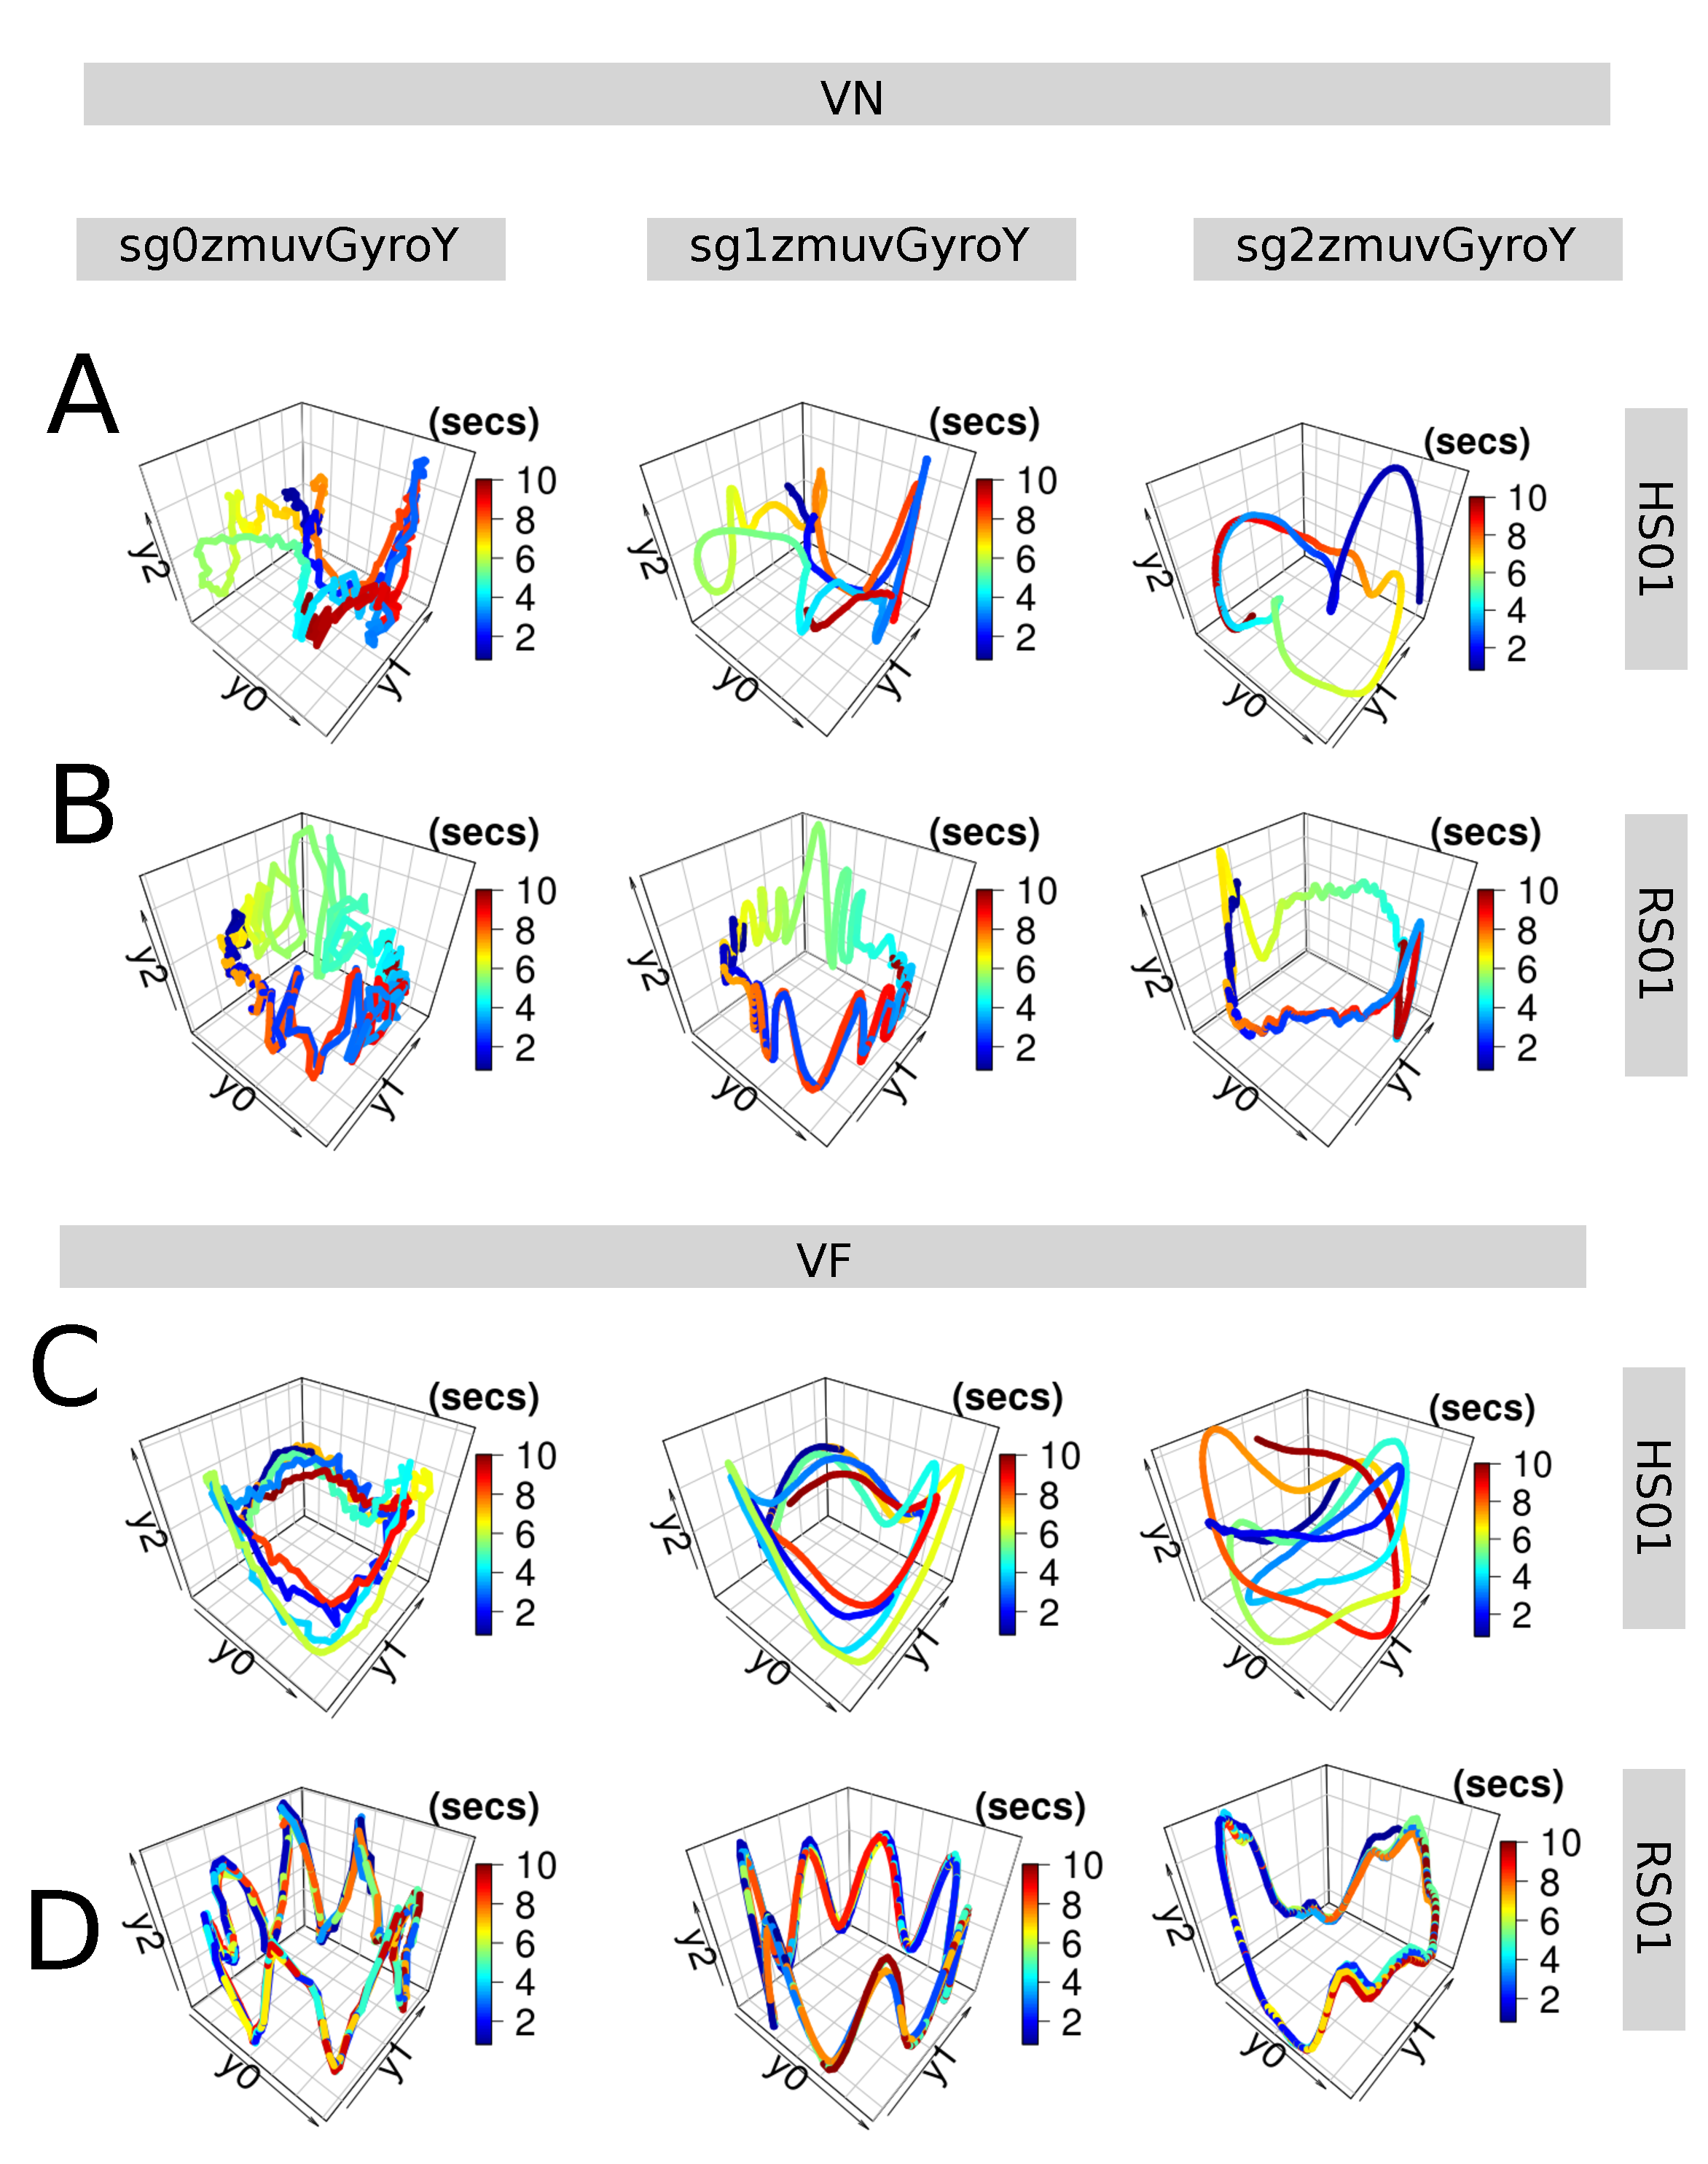
\includegraphics[height=0.85\textheight]{fig_6_05}
    \caption
	[RSSs for vertical arm movements]{
	{\bf RSSs for vertical arm movements.}
	Reconstructed state spaces %for time series of Figure \ref{fig:tsV}.
	of participant p01 for vertical movements in normal and faster 
	velocity (VN, VF) with raw-normalised (sg0zmuvGyroZ), 
	normalised-smoothed 1 (sg1zmuvGyroZ) and 
	normalised-smoothed 2 (sg2zmuvGyroZ) time series of the 
	sensors attached to the participant (HS01) and other sensor 
	attached to the robot (RS01).	
	Reconstructed state spaces were computed with 
	embedding parameters $\overline{m_0}=6$, $\overline{\tau_0}=8$.
	\R code to reproduce the figure is available at 
	\codelink{
	https://github.com/mxochicale-phd/thesis/tree/master/0_code_data/1_code/8_figs_ch6/03_fig6.4-6.5
	}.
        }
    \label{fig:rss_aVw10}
\end{figure}
%%---------------------------------(FIGURE)------------------------------------

Therefore, one can observe by eye the differences in each of the trajectories 
in the reconstructed state spaces 
(Figs~\ref{fig:rss_aHw10}, \ref{fig:rss_aVw10}), 
however one might be not objective when quantifying those differences 
since such observations might vary from person to person.
With that in mind, in early experiments of this thesis, 
it had been tried to objectively quantify those differences 
using euclidean distances between 
the origin to each of the points in the trajectories in the trajectories of 
the RSSs, however these created suspicious metrics, specially 
for trajectories which looked very messy.
Hence, it has been proposed the application of 
Recurrence Quantification Analyses (RQA) 
in order to have a more objective quantification of the differences 
in each of the cases of the time series.

\newpage
\section{Recurrences Plots}
Considering the time series of Figs~\ref{fig:tsH} and \ref{fig:tsV}, 
Recurrence Plots are computed for horizontal arm movements  
(Fig~\ref{fig:rp_aH}) and vertical arm movements (Fig~\ref{fig:rp_aV}) 
using the average embedding parameters 
($\overline{m_0}=6$, $\overline{\tau_0}=8$) 
and a recurrence threshold of $\epsilon=1$. 
For the selection of the recurrence threshold,
\cite{marwan2011} pointed out that choosing an appropriate 
recurrence threshold is crucial to get meaningful representations in the RPs, 
however, for this thesis where quantifying movement variability is our aim,
little importance has been given to the selection of the recurrence threshold 
for the RPs as long as it is able to represent the dynamical transitions 
in each of the time series.

In general, the increase of smoothness in time series results in thicker 
and better defined diagonal lines in the RPs 
(Figs~\ref{fig:rp_aH}, \ref{fig:rp_aV}).
Additionally, due to the changes in velocities of the movements 
the patterns in the RPs present an increase of diagonal lines 
and a decrease of line thickness.
%(Figs~\ref{fig:rp_aH}, \ref{fig:rp_aV}).
Although, the patterns of RPs show consistency with the movements type 
and velocities changes, it can be noticed that patterns of the RPs for 
HS01 are not well defined while patterns of the RPs for RS01 
shown a more consistent pattern (Fig~\ref{fig:rp_aH}, \ref{fig:rp_aV}). 

It is important to note that only RPs for participant 01 are presented
in (Fig~\ref{fig:rp_aV}, \ref{fig:rp_aH}), however
other RPs for all participants are presented in Appendix \ref{appendix:f:rps}.
With that in mind, it can be highlighted that, as similar as, the 
Reconstructed State Spaces (Figs~\ref{fig:rss_aHw10}, \ref{fig:rss_aVw10}), 
the patterns in the RPs can be easily noticed by eye for different conditions 
of the time series (Figs~\ref{fig:rp_aH}, Fig~\ref{fig:rp_aV}),
however these characteristics in the patterns of the RPs are subjective 
for the person who analysed them and might vary from person to person. 
That lead us to apply Recurrence Quantification Analysis (RQA) in order 
to have an objective quantification metric for the movement variability 
for each of the conditions of the time series.
%%---------------------------------(FIGURE)-------------------------------------
\begin{figure}
\centering
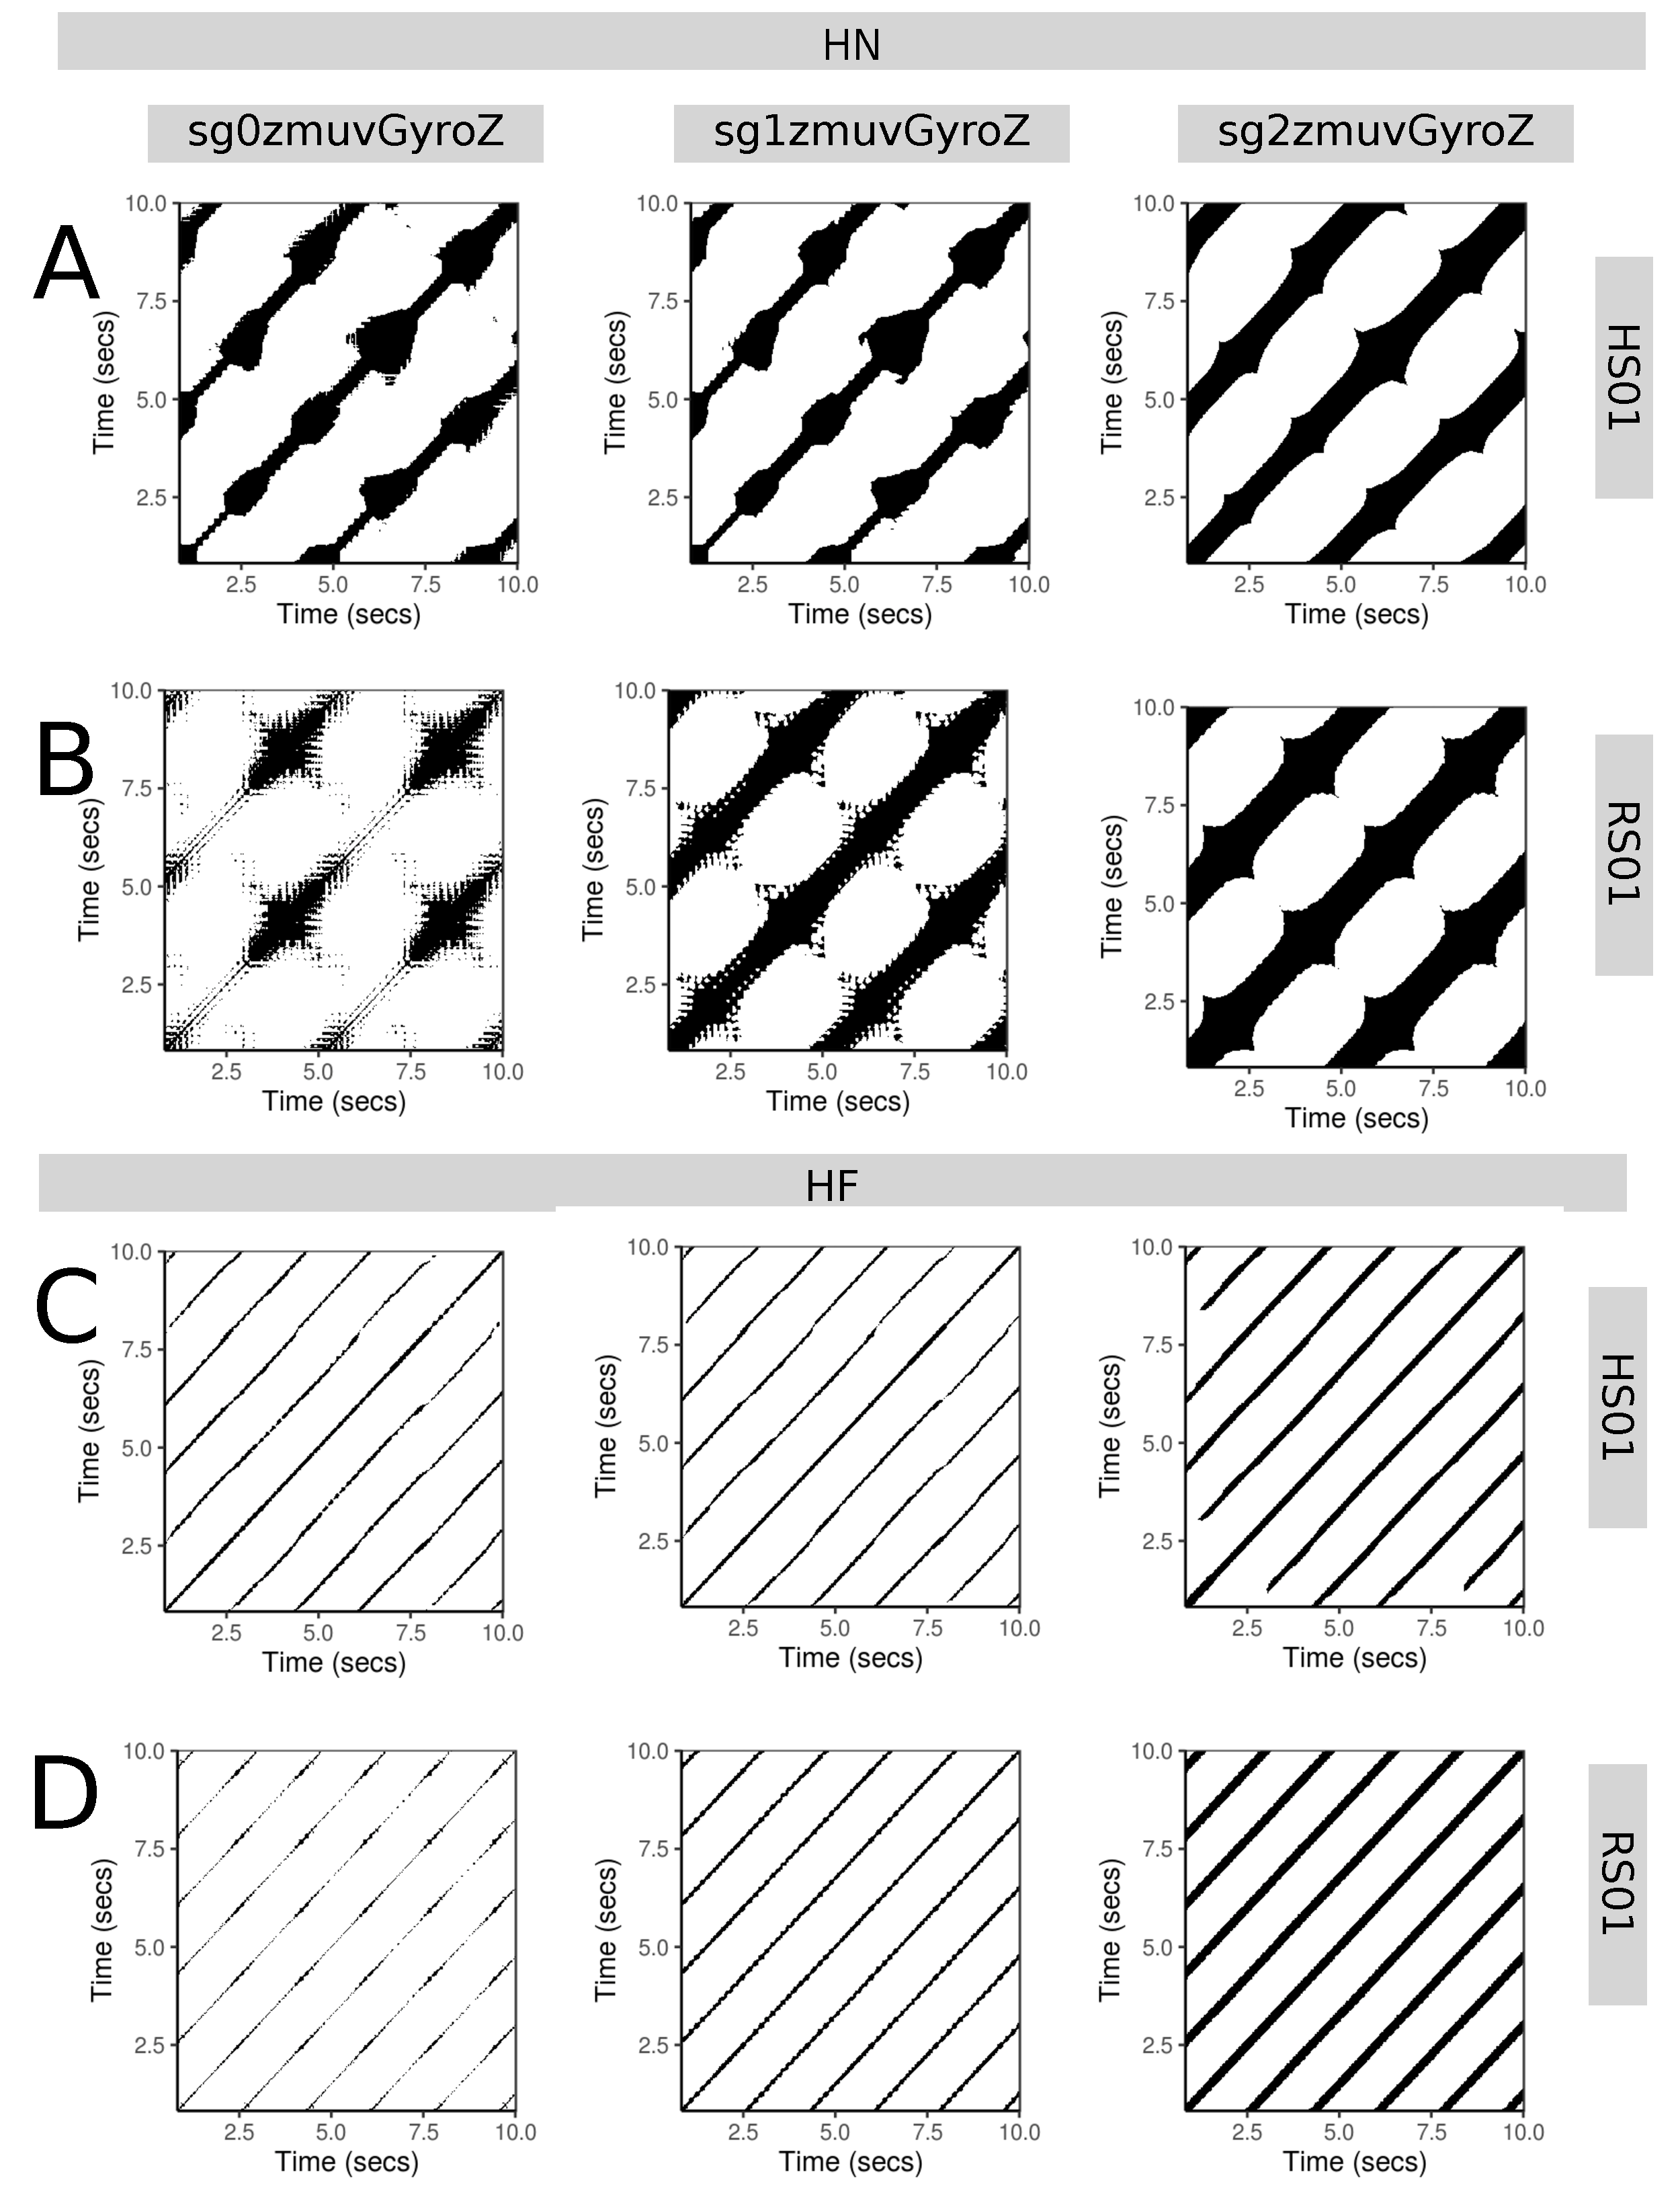
\includegraphics[height=0.80\textheight]{fig_6_06}
\caption
	[RPs for horizontal arm movements]{
	{\bf RPs for horizontal arm movements.}	
	Recurrence plots %for time series of Figure \ref{fig:tsV}.
	of participant $p01$ for horizontal movements in normal and faster 
	velocity (HN, HF) with time series of raw-normalised (sg0zmuvGyroZ), 
	normalised-smoothed 1 (sg1zmuvGyroZ) and 
	normalised-smoothed 2 (sg2zmuvGyroZ), and 
	sensors attached to the participant (HS01) and to the robot (RS01).
	Recurrence plots were computed with 
	embedding parameters $\overline{m_0}=6$, $\overline{\tau_0}=8$ and
	recurrence threshold $\epsilon=1$.
	\R code to reproduce the figure is available at 
	\codelink{
	https://github.com/mxochicale-phd/thesis/tree/master/0_code_data/1_code/8_figs_ch6/04_fig6.6-6.7/code
	}.
        }
    \label{fig:rp_aH}
\end{figure}
%%---------------------------------(FIGURE)------------------------------------
%%---------------------------------(FIGURE)-------------------------------------
\begin{figure}
\centering
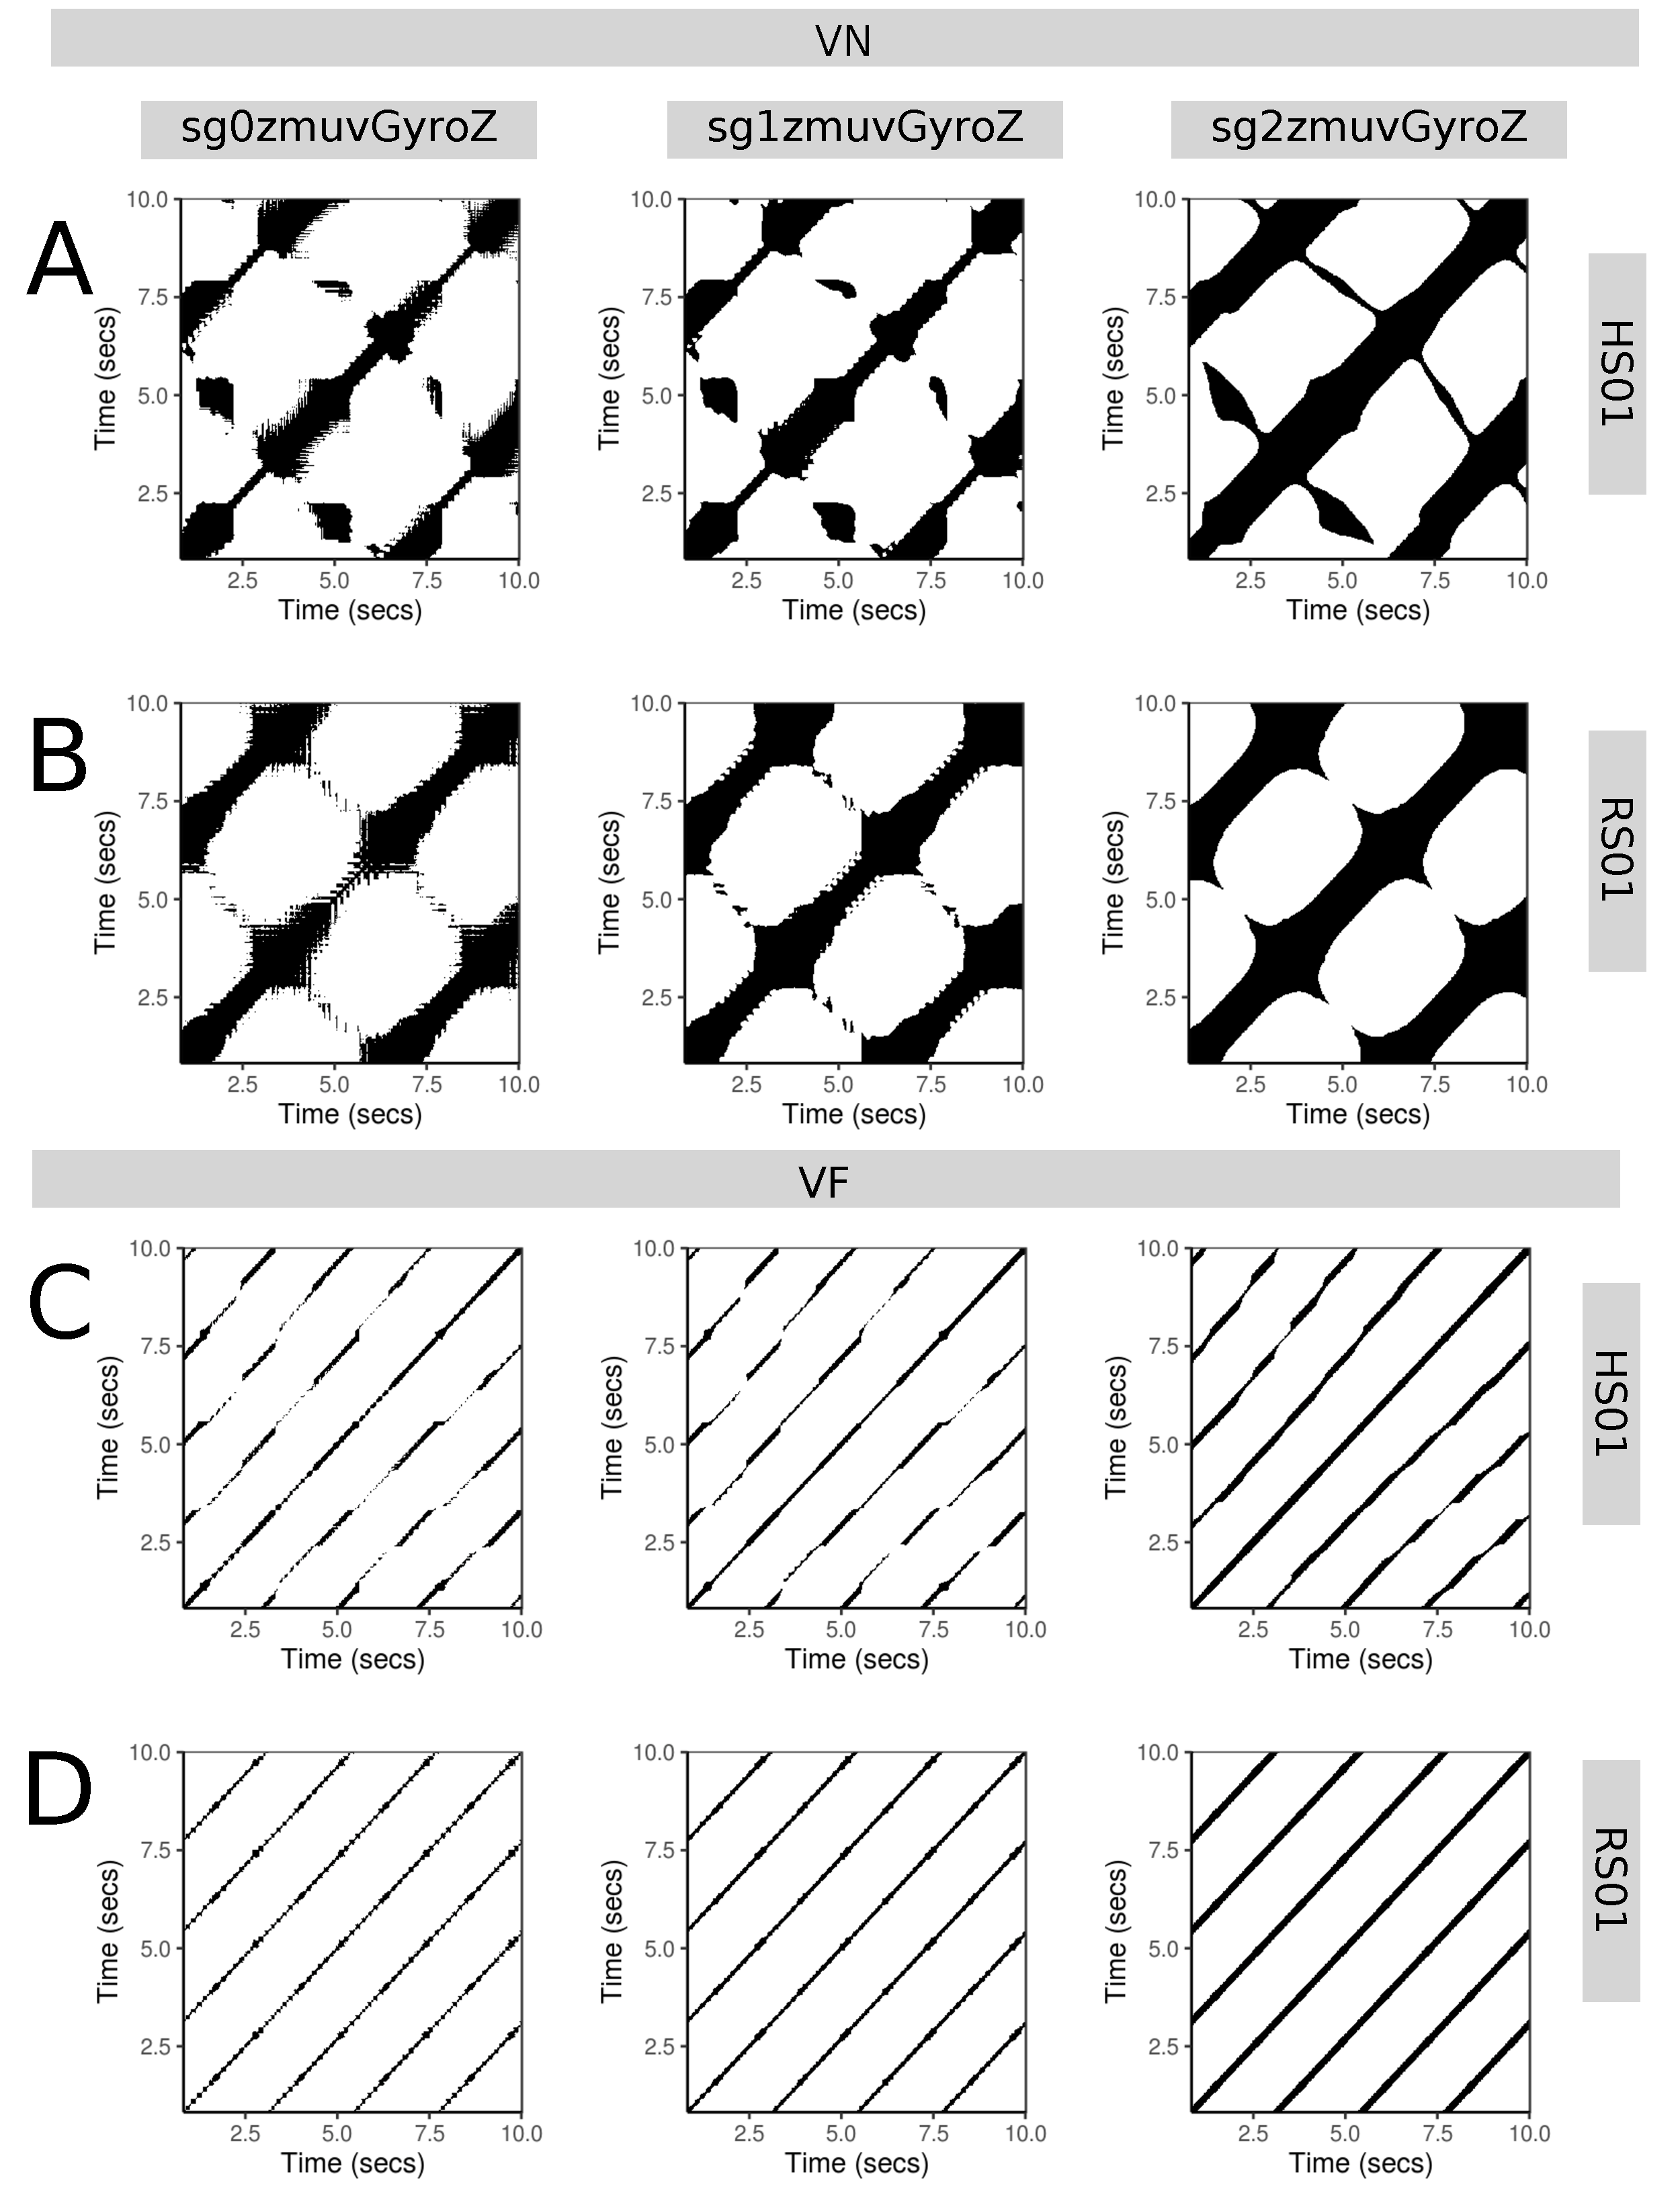
\includegraphics[height=0.80\textheight]{fig_6_07}
\caption
	[RPs for vertical arm movements]{
	{\bf RPs for vertical arm movements.}	
	Recurrence plots %for time series of Figure \ref{fig:tsV}.
	of participant $p01$ for vertical movements in normal and faster 
	velocity (VN, VF) with time series of raw-normalised (sg0zmuvGyroZ), 
	normalised-smoothed 1 (sg1zmuvGyroZ) and 
	normalised-smoothed 2 (sg2zmuvGyroZ), and 
	sensors attached to the participant (HS01) and to the robot (RS01).
	Recurrence plots were computed with 
	embedding parameters $\overline{m_0}=6$, $\overline{\tau_0}=8$ and
	recurrence threshold $\epsilon=1$.
	\R code to reproduce the figure is available at 
	\codelink{
	https://github.com/mxochicale-phd/thesis/tree/master/0_code_data/1_code/8_figs_ch6/04_fig6.6-6.7/code
	}.
        }
    \label{fig:rp_aV}
\end{figure}
%%---------------------------------(FIGURE)------------------------------------

\newpage
\section{Recurrence Quantification Analysis} \label{ch6:rqas}
Considering the RPs for 20 participants performing four activities 
(HN, HF, VN and VF) with sensors attached to the human (HS01) and to the 
humanoid robot (RS01) and with the increase of smoothness of time series 
(sg0zmuvGyroZ, sg1zmuvGyroZ and sg2zmuvGyroZ), 
I hence compute four metrics of RQA metrics (REC, DET, RATIO and ENTR) with 
embedding parameters $\overline{m_0}=6$, $\overline{\tau_0}=8$ and 
recurrence threshold $\epsilon=1$.
 
%\newpage
\subsection*{REC values}
It can be seen in the box plots of Figs~\ref{fig:RQABP}(A) that REC values, 
representing the \% of black dots in the RPs, 
are more spread for HN and VN movements (higher interquartile range) 
than HF and VF movements (lower interquartile range) for HS01 sensor. 
In contrast, REC values for RS01 sensor present little variation 
(interquartile range of 0.01).
With regard to the increase of smoothness of time series 
(sg0, sg1 and sg2), REC values present little 
variation as the smoothness is increasing for time series from HS01 
(changes of mean values (rhombus)) while REC values are more affected with 
the smoothness for data from RS01 
(see the incremental changes of mean values (rhombus)).
See Figs~\ref{fig:rec_aH} and \ref{fig:rec_aV} in Appendix \ref{appendix:f:rqas} 
for more details about individual REC values for each participant.

\subsection*{DET values}
Figs \ref{fig:RQABP}(B) illustrate DET values, 
representing predictability and organisation of the RPs, 
which change very little (interquartile range is around 0.1) 
for type of movement, level of smoothness or type of sensor.
See Figs~\ref{fig:det_aH} and \ref{fig:det_aV} in Appendix \ref{appendix:f:rqas} 
for more details about individual DET values for each participant.

\subsection*{RATIO values}
Figs \ref{fig:RQABP}(C) present RATIO values, representing dynamic transitions, 
for horizontal and vertical movements.
It can be seen that RATIO values for HS01 sensor vary less 
for HN movements (interquartile range around 2)
than HF movements (interquartile range around 5).
%which is a similar behaviour of RATIO values for oRS01 sensor.
It can also be noticed a decrease of variation in RATIO values as the 
smoothness of the time series is increasing (grey rhombus).
See Figs~\ref{fig:ratio_aH} and \ref{fig:ratio_aV} in Appendix 
\ref{appendix:f:rqas} 
for more details about individual RATIO values for each participant.

\subsection*{ENTR values}
Fig. \ref{fig:RQABP}(D) show ENTR values, representing the complexity of 
the structure the time series, for both horizontal and vertical movements.
ENTR values for HS01 sensor show more variation 
(interquartile range around 0.5)
than ENTR values for RS01 sensor which appear 
to be more constant (interquartile range 0.1).
It can also be said that the smoothness of time series affects
each of the axis by an increase of mean values (see gray rhombos).
See Figs~\ref{fig:entr_aH} and \ref{fig:entr_aV} in Appendix
\ref{appendix:f:rqas}
for more details about individual ENTR values for each participant.

%%---------------------------------(FIGURE)-------------------------------------
\begin{figure}
\centering
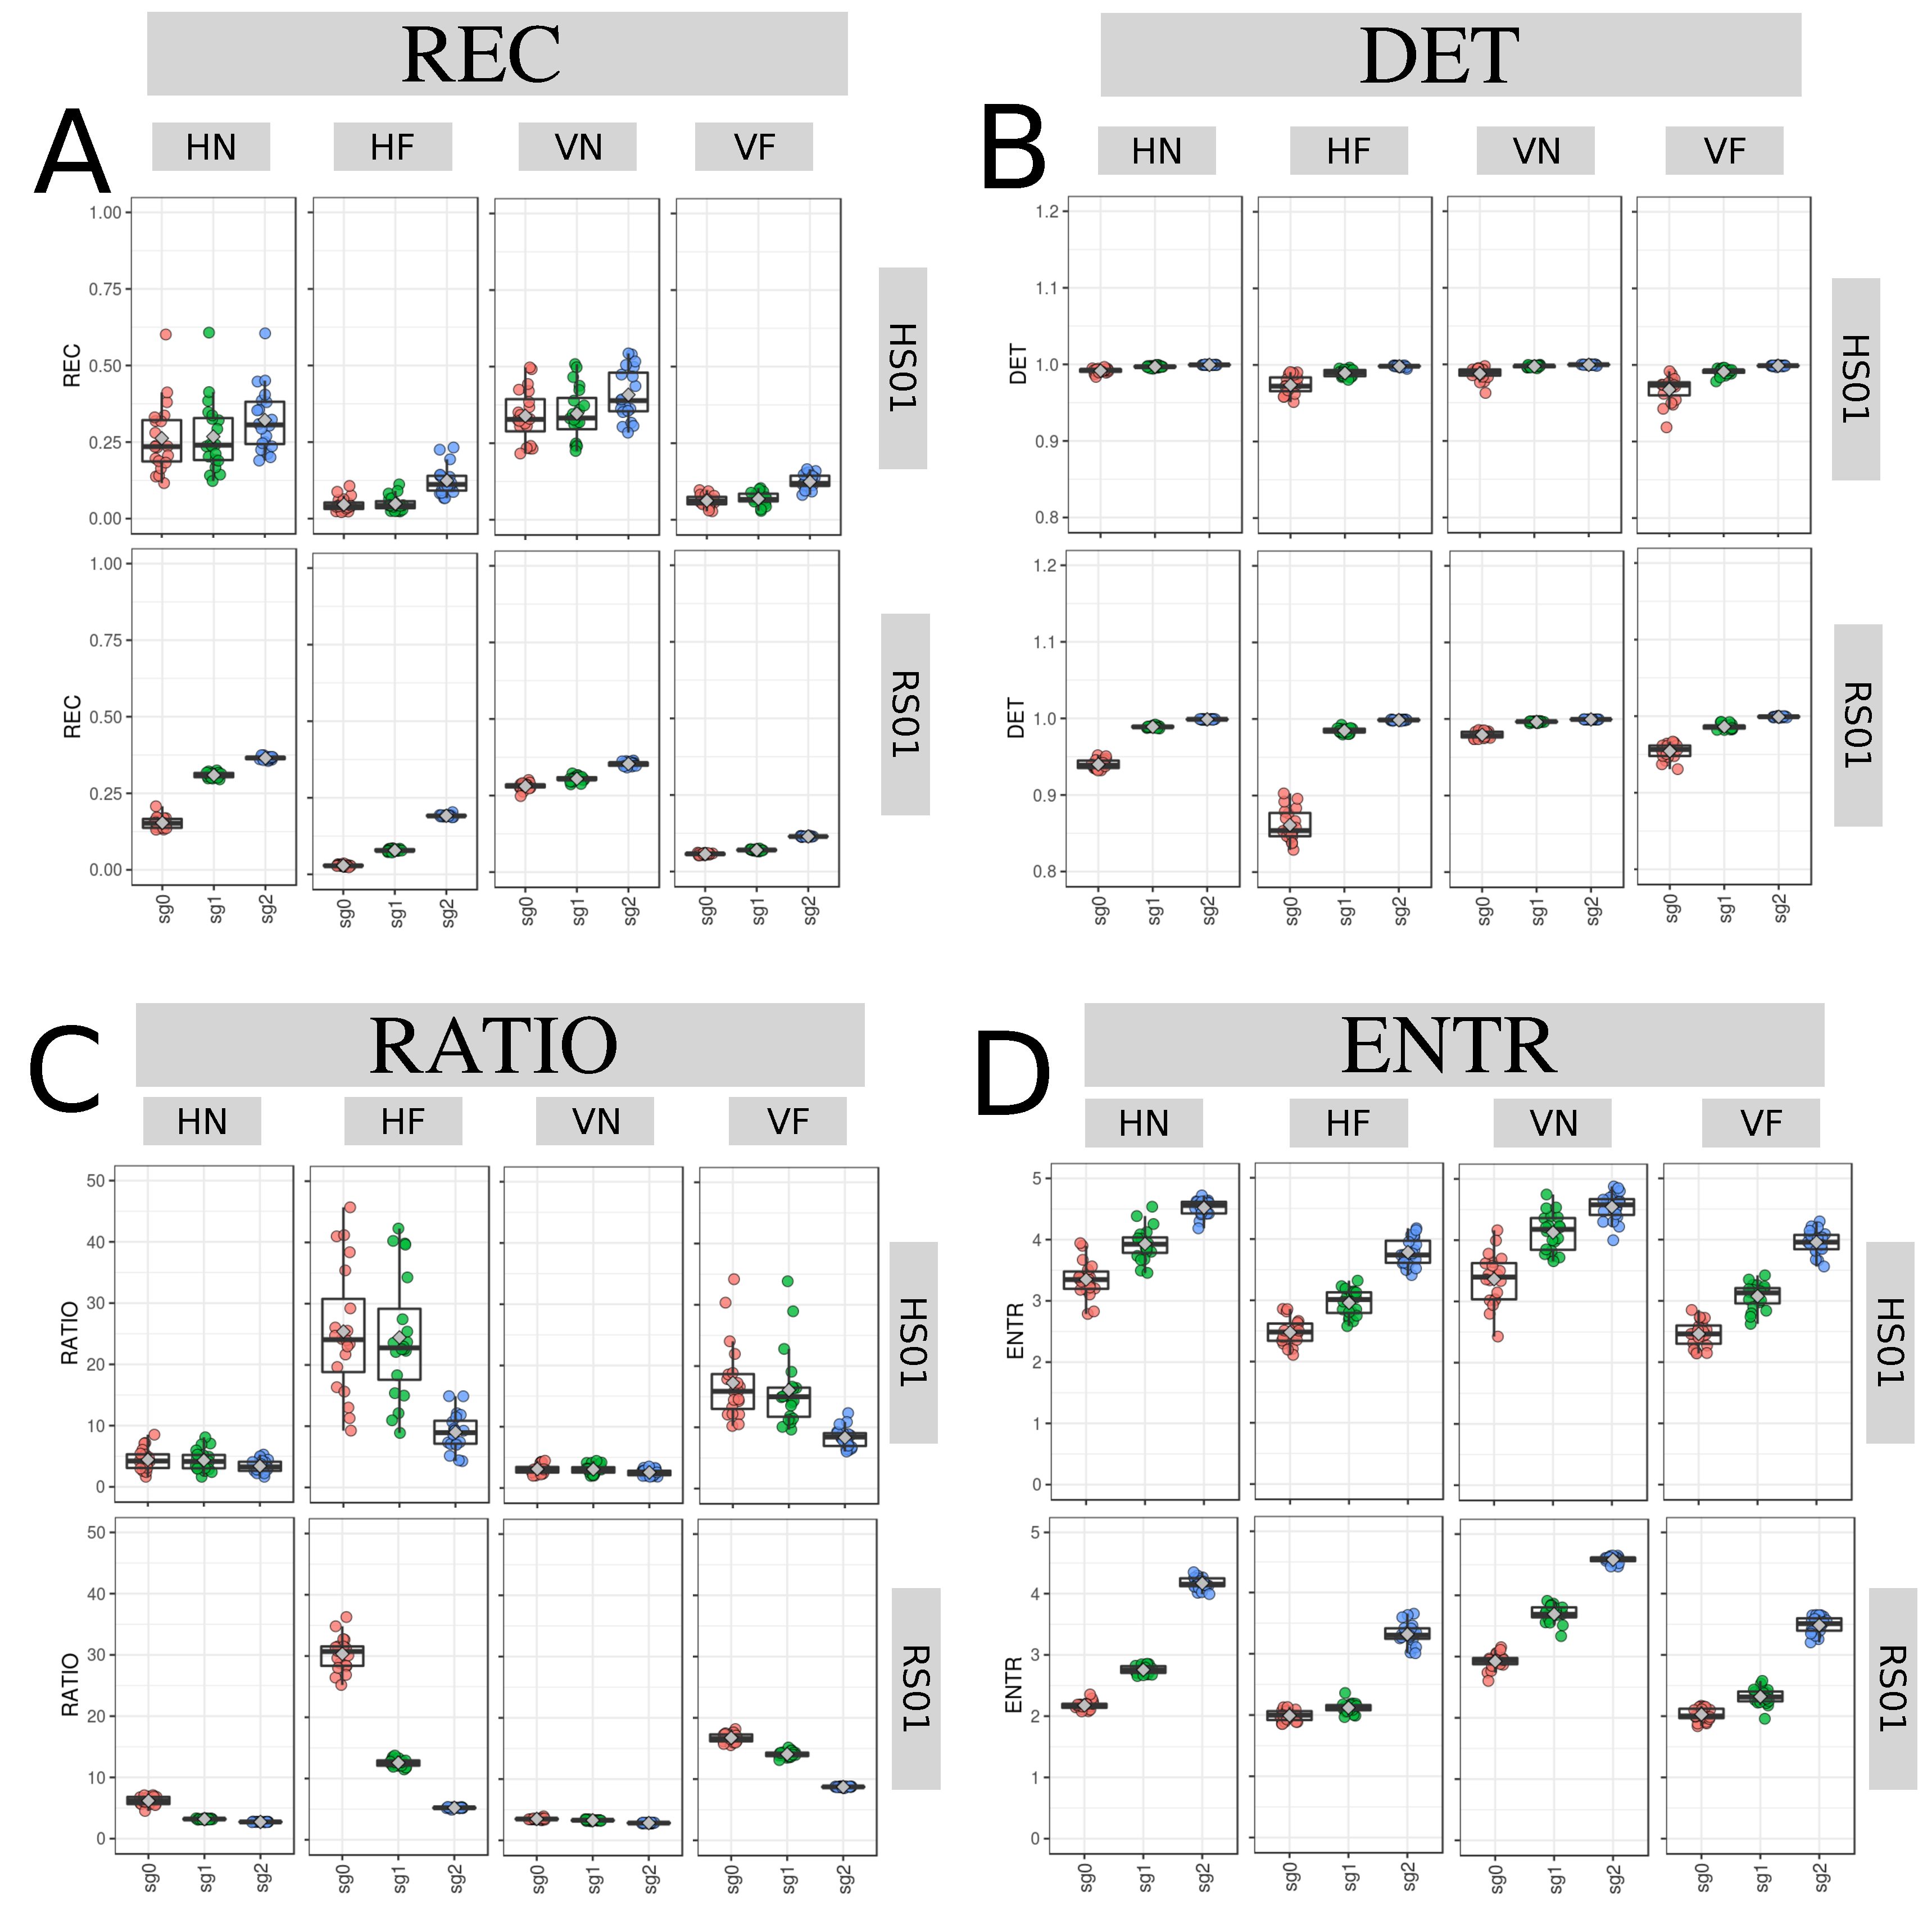
\includegraphics[width=1.0\textwidth]{fig_6_08}
    \caption
	[Box plots for RQA values]{
	{\bf Box plots for RQA values.}
	Box plots of (A) REC, (B) DET, (C) RATIO, and (D) ENTR values 
	for 20 participants performing HN, HF, VN and VF movements
	with sensors HS01, RS01 and three smoothed-normalised  
	time series (sg0, sg1 and sg2).
	RQA values were computed with 
	embedding parameters $\overline{m_0}=6$, $\overline{\tau_0}=8$ and
	recurrence threshold $\epsilon=1$.
	\R code to reproduce the figure is available at 
	\codelink{
	https://github.com/mxochicale-phd/thesis/tree/master/0_code_data/1_code/8_figs_ch6/05_fig6.8/code	
	}.
        }
    \label{fig:RQABP}
\end{figure}
%%---------------------------------(FIGURE)------------------------------------

\newpage
\section{Weaknesses and strengths of RQA}
Considering the Section \ref{sec:ws_rqa} regarding 
the weaknesses and strengths of RQA, 
RQA metrics (i.e., REC, DET, RATIO and ENTR) 
are computed and plotted 3D surface plots using an unitary 
increase of pair embedding parameters 
($0 > m \le 10$, $0 > \tau \le 10$) 
and a decimal increase of 0.1 for recurrence thresholds 
($ 0.2 \ge \epsilon \le 3 $) (Fig.~\ref{fig:topo_rqas}). 
Hence, Fig.~\ref{fig:topo_rqas}(A) shows an increase for 
REC values, the percentage of black dots in the RP, 
as the recurrence threshold increases,
while the variation for embedding parameters creates little decrease 
of REC values as the embedding dimensions increase and even slighter 
decrements of REC values for the increase of $\tau$.
For the 3D surface plots of DET values (Fig.~\ref{fig:topo_rqas}(B)), 
representing 
predictability and organisation of the RPs, one can note a plateau
for DET values near to 1 for embedding dimension parameters of less 
than 5 and recurrence threshold values of greater than 2 (red surface). 
It can also be observed that the increases of delay embedding made 
the DET values increase so as to make an cascade effect in the surface 
along with the increase of dimension embedding $m$.
For RATIO values, representing dynamic transitions, 
Fig.~\ref{fig:topo_rqas} shows that the 3D surface plots present 
a plateau (blue surface) of RATIO values 
near to zero for recurrence thresholds greater than 1.0, while 
fluctuations are more evident for recurrence thresholds of less than 1.0,
particularly it can also be noted an increase in the fluctuations of 
RATIO values as the embedding dimension is increasing. 
For ENTR values in Fig.~\ref{fig:topo_rqas}(D), 
representing the complexity of the structures in time series, 
one can note that the increase of recurrence threshold is, 
not strictly proportional to the increase of ENTR values. 
It can also be observed in Fig.~\ref{fig:topo_rqas}(D)
that the increase of delay embeddings hardly affects 
the ENTR values for embedding dimensions of 1, while 
for higher values of embedding dimensions 
there is a decrease of ENTR values, and 
there is a decrease of ENTR values as delay dimension value is increasing.
%---------------------------------(FIGURE)-------------------------------------
\begin{figure}
\centering
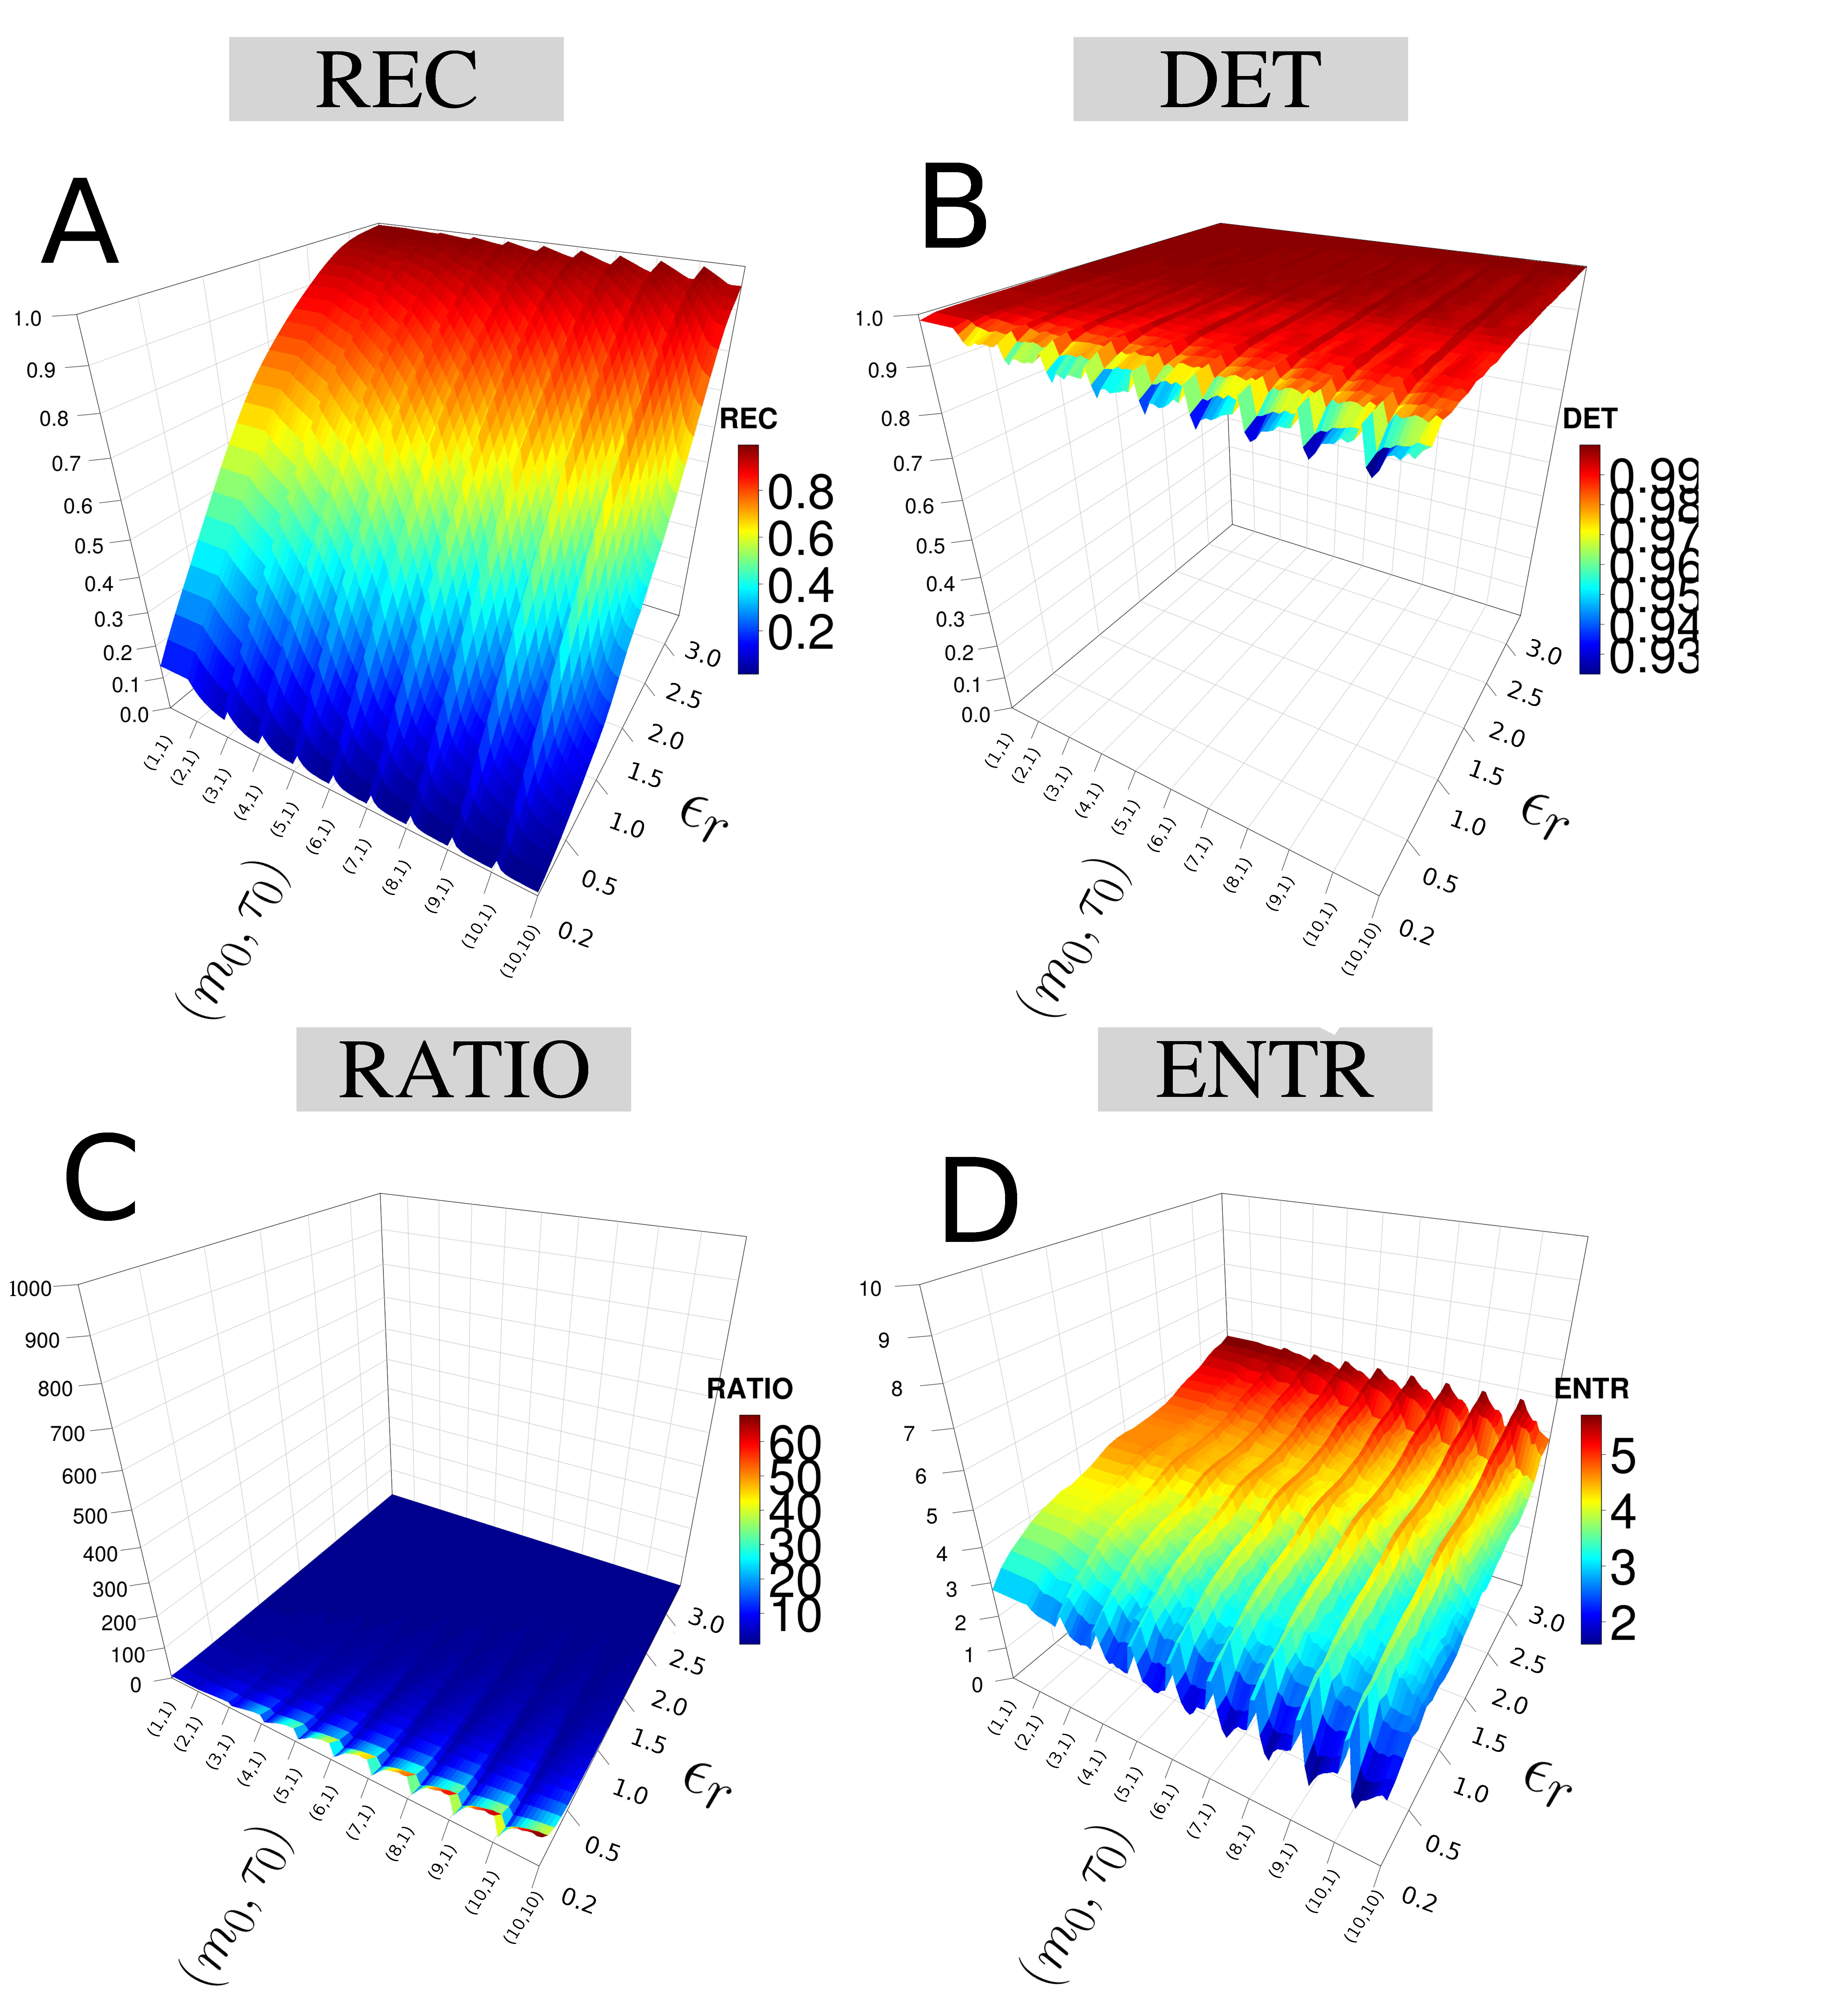
\includegraphics[width=1.0\textwidth]{fig_6_09}
    \caption
	[3D surface plots for RQA metrics]{
	{\bf 3D surface plots for RQA metrics.}
	3D surface plots for (A) REC, (B) DET, (C) RATIO and (D) ENTR values 
	with increasing pair of embedding parameters 
	($0 \le m \le 10$, $0 \le \tau \le 10$) 
	and recurrence thresholds (  $ 0.2 \le \epsilon \le 3 $).
	RQA metrics are computed with the time series of participant $p01$ using 
	HS01 sensor, HN activity, sg0zmuvGyroZ axis and 10 seconds 
	for window length.
 	\R code to reproduce the figure is available at 
	\codelink{
	https://github.com/mxochicale-phd/thesis/tree/master/0_code_data/1_code/8_figs_ch6/06_fig6.9/code	
	}.
	}
\label{fig:topo_rqas}
\end{figure}
%---------------------------------(FIGURE)------------------------------------

\newpage
\subsection{Sensors and activities}
We also computed 3D surface plots of RQA metrics for different sensors 
and different activities 
(Figs.~\ref{fig:topo_sa_hs01}, \ref{fig:topo_sa_rs01}), where it can 
generally be noted similar 3D surface plots patterns for RQA metrics as the ones
in Fig. \ref{fig:topo_rqas}. 

The 3D surface plots for REC values (Fig. \ref{fig:topo_sa_hs01}(A))
show slightly differences with regard to vertical or horizontal activities
however there are notable differences for normal and faster velocities, 
specially for the faster movements where the 3D surface plots shows a maximum
REC value for embedding dimension values near to 1 and for recurrence 
thresholds near to 3. 
The 3D surface plots of DET values  
(Fig. \ref{fig:topo_sa_hs01}(B)) and RATIO values 
(Fig. \ref{fig:topo_sa_hs01}(C)) show slightly notable variations across 
the type of activities. 
For 3D surface plots of ENTR values it can be noted a slightly variation for
surface plots of normal and faster velocities (Fig \ref{fig:topo_sa_hs01}(D)).
%%---------------------------------(FIGURE)-------------------------------------
\begin{figure}
\centering
\includegraphics[width=1.0\textwidth]{fig_6_10}
    \caption
	[3D surface plots of RQA metrics for HS01 sensor]{
	{\bf 3D surface plots of RQA metrics for HS01 sensor.}
	3D surface plots of RQA metrics ((A) REC, (B) DET, (C) RATIO, and (D) ENTR) 
	with increasing embedding parameters and recurrence thresholds 
	are for time series of participant $p01$ for 
	sensors HS01, activities (HN, HF, VN and VF) and 
	sg0zmuvGyroZ axis with 10 seconds window length. 
	\R code to reproduce the figure is available at 
	\codelink{
	https://github.com/mxochicale-phd/thesis/tree/master/0_code_data/1_code/8_figs_ch6/07_fig6.10-6.11/code
	}.
       }
\label{fig:topo_sa_hs01}
\end{figure}
%---------------------------------(FIGURE)-------------------------------------

As similar as Fig \ref{fig:topo_sa_hs01}, the 3D surface plots patters 
for RS01 in Fig \ref{fig:topo_sa_rs01} show the differences between 
the activities performed at normal and faster velocities
specially for REC and ENTR values (Fig \ref{fig:topo_sa_hs01}(A, D)),
while 3D surface plots for DET and RATIO values show slightly variations
(Fig \ref{fig:topo_sa_hs01}(B, C)).
%%---------------------------------(FIGURE)-------------------------------------
\begin{figure}
\centering
\includegraphics[width=1.0\textwidth]{fig_6_11}
    \caption
	[3D surface plots of RQA metrics for RS01 sensor]{
	{\bf 3D surface plots of RQA metrics for RS01 sensor.}
	3D surface plots of RQA metrics ((A) REC, (B) DET, (C) RATIO and (D) ENTR) 
	with increasing embedding parameters and recurrence thresholds 
	are for time series of humanoid robot for 
	sensors RS01, activities (HN, HF, VN and VF) and 
	sg0zmuvGyroZ axis with 10 seconds window length. 
	\R code to reproduce the figure is available at 
	\codelink{
	https://github.com/mxochicale-phd/thesis/tree/master/0_code_data/1_code/8_figs_ch6/07_fig6.10-6.11/code
	}.
       }
\label{fig:topo_sa_rs01}
\end{figure}
%---------------------------------(FIGURE)-------------------------------------

%\newpage
\subsection{Window size}
Figs.~\ref{fig:topo_windows} illustrate 3D surface plots for RQA metrics 
with four window lengths of 2-sec, 5-sec, 10-sec, and 15-sec.
In general, it can be said that the increase of window length 
of the time series creates 3D surface plots patterns with better resolution.
%Figs. \ref{fig:topo_windows} 
%---------------------------------(FIGURE)-------------------------------------
\begin{figure}
\centering
\includegraphics[width=1.0\textwidth]{fig_6_12}
    \caption
	[3D surface plots of RQAs metrics with four window lengths]{
	{\bf 3D surface plots of RQAs metrics with four window lengths.}
	3D surface plots of RQA metrics ((A) REC, (B) DET, (C) RATIO, and (D) ENTR) 
	with increasing embedding 
	parameters and recurrence thresholds for four window 
	lengths (w2-sec, w5-sec, w10-sec and w15-sec).
	RQA metrics values are for time series of participant $p01$ 
	using HS01 sensor, HN activity and sg0zmuvGyroZ axis.
	\R code to reproduce the figure is available at 
	\codelink{
	https://github.com/mxochicale-phd/thesis/tree/master/0_code_data/1_code/8_figs_ch6/08_fig6.12/code
        }.
	}
\label{fig:topo_windows}
\end{figure}
%%---------------------------------(FIGURE)------------------------------------

\newpage
\subsection{Smoothness}
Figs \ref{fig:topo_smoothness} present 3D surface plots of the RQA metrics
considering three levels of smoothness of the time series (sg0, sg1, sg2).
It can then be noted that such smoothness have a direct effect on the 
smoothness of the 3D surface plots.
Especially for dimension embeddings lower than 2 with in REC and ENTR values 
(Fig.~\ref{fig:topo_smoothness}(A, D)).
The 3D surface plots of DET values are smoothed to a degree that the plateau 
(red surface) is increase, while RATIO values appear to be less 
affected to the level of smoothness (Fig.~\ref{fig:topo_smoothness}(C)).
%%---------------------------------(FIGURE)-------------------------------------
\begin{figure}
\centering
\includegraphics[width=1.0\textwidth]{fig_6_13}
    \caption
	[3D surface plots of RQA metrics with three levels of smoothness]{
	{\bf 3D surface plots of RQA metrics with three levels of smoothness.}
	3D surface plots of RQA metrics ((A) REC, (B) DET, (C) RATIO, and (D) ENTR) 
	with increasing embedding parameters and recurrence thresholds for 
	three levels of smoothness 
	(sg0zmuvGyroZ, sg1zmuvGyroZ and sg1zmuvGyroZ).
	RQA metrics are computed from time series of participant $p01$ using 
	HS01 sensor, HN activity and 10 seconds window length.
	\R code to reproduce the figure is available at 
	\codelink{
	https://github.com/mxochicale-phd/thesis/tree/master/0_code_data/1_code/8_figs_ch6/09_fig6.13/code        
	}.
 	}
\label{fig:topo_smoothness}
\end{figure}
%%---------------------------------(FIGURE)------------------------------------

\subsection{Participants}
Figs ~\ref{fig:topo_participants} illustrate 3D surface plots of RQA metrics for 
four participants.
It can be noted that differences of the 3D surface plots across participants 
are more notable with REC (Fig.~\ref{fig:topo_participants}(A)) and 
ENTR values (Fig.~\ref{fig:topo_participants}(D)),
while minor differences of 3D surface plots across participants are 
presented in
DET (Fig.~\ref{fig:topo_participants}B)) and 
RATIO vales (Fig.~\ref{fig:topo_participants}(C)).
%%---------------------------------(FIGURE)-------------------------------------
\begin{figure}
\centering
\includegraphics[width=1.0\textwidth]{fig_6_14}
    \caption
	[3D surface plots of RQA metrics with three participants]{
	{\bf 3D surface plots of RQA metrics with three participants.}
	3D surface plots of RQA metrics ((A) REC, (B) DET, (C) RATIO, and (D) ENTR) 
	for participants $p01$, $p02$, $p03$ and $p04$ with increasing embedding 
	parameters and recurrence thresholds.
	RQA metrics values are for time series of HS01 sensor, 
	HN activity and 10 seconds window length.
	\R code to reproduce the figure is available at 
	\codelink{
	https://github.com/mxochicale-phd/thesis/tree/master/0_code_data/1_code/8_figs_ch6/10_fig6.14/code
	}.
 }
\label{fig:topo_participants}
\end{figure}
%%---------------------------------(FIGURE)-------------------------------------

\newpage
\subsection{Final remarks}
It can be noted that the changes of RQA metrics are evident
with both the increase of embedding dimension parameters and the 
recurrence threshold for different structures, window size, 
levels of smoothness of the time series. 
For instance, RATIO values present a plateau (blue colour surface) 
which is independently to the source of time series, 
however there are peaks that change 
differently based on the source of time series. 
%for increasing 
%embedding parameters  with recurrence threshold less than one.
For DET values, 3D surface plots present a fluctuated surface (red colour)
which slightly differs with the source of time series.
With regards to REC values, 3D surface plots are affected by the velocity
of movements. For example, surface plots for normal velocity presents 
an increase of REC values as recurrence threshold increases and 
keeping slightly uniform surface plot changes for the increase 
of embedding parameters.
However for faster velocity arm movements, 3D surface plot fluctuations 
decrease as the embedding dimension increases and 
recurrence thresholds increases.
Similarly as the results of human-image activities  
(see Section \ref{wsRQAhii} in Chapter \ref{chapter5}), 
3D surface plots of ENTR values for human-humanoid interaction  
present changes to any of the types of time series 
which might be of help to understand 
the dynamics of 
movement variability in human-humanoid activities
from different time series.

